\documentclass[12pt, a4paper]{article}

\usepackage[utf8]{inputenc}
\usepackage[T1]{fontenc}
\usepackage[margin=1.2in]{geometry}
\usepackage{setspace}
\usepackage{amsmath, amssymb, amsthm}
\usepackage{mathtools}
\usepackage{thmtools}
\usepackage{natbib}
\usepackage{hyperref}
\usepackage{xcolor}
\usepackage{booktabs}
\usepackage{array}
\usepackage{longtable}
\usepackage{enumitem}
\usepackage{epigraph}
\usepackage{titlesec}
\usepackage{fancyhdr}
\usepackage{abstract}
\usepackage{tikz}
\usetikzlibrary{arrows.meta, positioning, calc}

\hypersetup{
  colorlinks=true,
  linkcolor=black,
  citecolor=black,
  urlcolor=black
}

\onehalfspacing

\titleformat{\section}{\large\bfseries}{\thesection.}{1em}{}
\titleformat{\subsection}{\normalsize\bfseries}{\thesubsection.}{1em}{}
\titleformat{\subsubsection}{\normalsize\itshape}{\thesubsubsection.}{1em}{}

\pagestyle{fancy}
\fancyhf{}
\rhead{\small\textit{Frozen Processes}}
\lhead{\small Flyxion}
\cfoot{\thepage}
\renewcommand{\headrulewidth}{0.4pt}

\theoremstyle{plain}
\newtheorem{theorem}{Theorem}[section]
\newtheorem{lemma}[theorem]{Lemma}
\newtheorem{proposition}[theorem]{Proposition}
\newtheorem{corollary}[theorem]{Corollary}

\theoremstyle{definition}
\newtheorem{definition}[theorem]{Definition}
\newtheorem{example}[theorem]{Example}
\newtheorem{principle}[theorem]{Principle}

\theoremstyle{remark}
\newtheorem{remark}[theorem]{Remark}
\newtheorem{observation}[theorem]{Observation}

\setlength{\epigraphwidth}{0.65\textwidth}
\renewcommand{\epigraphflush}{center}

% -------------------------------------------------------
\begin{document}
% -------------------------------------------------------

\begin{titlepage}
\centering
\vspace*{2.5cm}
{\LARGE\bfseries Frozen Processes\\[0.6em]
\large Admissibility Structures, Trajectories, and Stable Residues:\\
A Framework for Process-Primary Theorizing\par}
\vspace{2.5cm}
{\large Flyxion}\\[0.5em]
{\normalsize Independent Research}\\[1em]
{\normalsize June 2026}
\end{titlepage}

% Abstract on its own page
\newpage
\thispagestyle{empty}
\begin{center}
{\large\bfseries Abstract}
\end{center}
\vspace{0.5em}
\noindent
This paper proposes a general explanatory framework organized around three
interlocking concepts: the \emph{admissibility structure} that determines
which transitions are possible in a given context, the \emph{trajectory}
through that structure, and the \emph{stable residue} that a trajectory
produces when it dwells within a bounded region long enough to be labeled.
The central claim is that what appear to be foundational entities are almost
always stable residues, and that the primary question about any configuration
is not ``does it exist?'' but ``is it reachable, and under what conditions
does it remain reachable?''

The paper motivates this framework by identifying a recurring structural error
across multiple disciplines---the \emph{Noun Fallacy}---in which a stable
residue is treated as a primitive, severing it from the trajectory and
admissibility structure that produced it. This error is not a simple mistake
but a rational consequence of the cognitive economy of compression, which
makes it persistent. It has been independently corrected in evolutionary
biology (species essentialism to population dynamics), thermal physics
(caloric fluid to kinetic theory), quantum field theory (particles to field
excitations), computation (object hierarchies to process calculi), urban
planning (master plans to generative sequences), and cognitive science
(stored representations to active inference trajectories). Each correction
exhibits the same structural move.

The paper develops eight major movements: an account of why compression
into nouns is rational and therefore persistent; a survey of independent
corrections across five domains; development of the general framework with
formal definitions and the \emph{Trajectory Compression Principle}; the
\emph{Reachability Ontology} as a named thesis; a case study in
re-nominalization using the software industry's misreading of Christopher
Alexander; an account of difficulty as a relational rather than intrinsic
property, including Goodhart dynamics as a re-nominalization mechanism;
a defense of process-primary theorizing as a methodological discipline;
and the \emph{Admissibility Log}---a proposed representational architecture
that stores changes in reachability rather than sequences of states, together
with a formal comparison to existing systems (Git, event sourcing, CRDTs,
process mining) and a worked demonstration of what each cannot express.
The paper concludes with a diagnostic appendix: five operational tests by
which any proposed primitive can be examined for the Noun Fallacy.

\newpage

\tableofcontents
\newpage

%%%%%%%%%%%%%%%%%%%%%%%%%%%%%%%%%%%%%%%%%%%%%%%%%%%%%
\section{Introduction: The Stability That Was Never There}
%%%%%%%%%%%%%%%%%%%%%%%%%%%%%%%%%%%%%%%%%%%%%%%%%%%%%

\epigraph{\textit{You cannot step into the same river twice.}}{Heraclitus, fr.\ 91}

\noindent
There is a tendency, so pervasive as to be nearly invisible, to treat the
outputs of ongoing processes as though they were the inputs to explanation.
A species is given as a fixed natural kind, and biology proceeds to ask how
such kinds interact, reproduce, and go extinct---without first asking what
population dynamics, selective pressures, and genetic processes constitute
the species as the apparently stable entity that classification requires.
A corporation is given as a legal person, and economics proceeds to model
its preferences---without asking what contractual, financial, and personnel
flows constitute the apparent coherence labeled by the corporate name.
A mental state is given as a representation, and cognitive science asks how
representations are stored and retrieved---without asking what sustained
neural activity constitutes the appearance of storage.

In each case, the nominal entity is real enough at a certain scale of
description. Species do differ reproducibly. Corporations do exhibit
behavioral regularities. Mental states do recur. The error is not in
recognizing these regularities but in treating them as primitives---as
bedrock from which explanation should proceed---rather than as precipitates
of processes that are themselves more fundamental, and that continue to
produce, sustain, and eventually dissolve the apparent entities.

This paper calls that error the \emph{Noun Fallacy}. The name is deliberately
informal. The point is not primarily grammatical---not a complaint about the
nouns language uses---but ontological and methodological: it concerns what
gets treated as basic in explanatory practice, and what gets obscured when
that choice is made carelessly. The Noun Fallacy occurs when a stabilized
trajectory through a space of admissible configurations is mistaken for a
fundamental entity, and when that mistaken identification propagates into the
theoretical architecture built on top of it.

The claim is not that nouns are wrong. The noun ``river'' is not wrong.
It is a useful compression of an ongoing hydrological process. The compression
becomes a fallacy when someone asks: what is the essential nature of the
river?---as though the answer could be given by examining the river apart
from the gravitational gradients, the precipitation patterns, the geological
substrates, and the erosion dynamics that constitute its existence as a river.
To treat the noun as a primitive is to ask a question whose very form
forecloses the informative answer.

What makes the Noun Fallacy persistent is that it is not a simple mistake.
It is the rational exploitation of a genuine cognitive economy. Compression
into stable labels is cheap. The compressed label permits coordination among
agents who would otherwise need to renegotiate every interaction from scratch.
The label ``river'' allows planning, navigation, and communication that would
be impossibly expensive if every use required reconstructing the hydrological
process from first principles. The compression earns its keep. The fallacy
occurs one step later, when the compression is mistaken for a description of
what is ultimately real, rather than for what it is: a lossy encoding of a
trajectory that remains in motion beneath the label.

This paper is organized around three interlocking theses.

The first is \emph{descriptive}: the Noun Fallacy has been independently
corrected, again and again, across biology, physics, computer science,
architecture, and cognitive science---not because investigators in those
fields coordinated, but because the same structural pressure eventually makes
the same error visible. Species essentialism gave way to population genetics.
Caloric fluid gave way to molecular kinetics. Static object hierarchies in
software gave way to functional composition, process calculi, and dataflow
networks. Master-planned urbanism gave way to generative urbanism.
Each of these transitions recovers a process from a nominal entity.

The second thesis is \emph{structural}: these independent corrections share
a common mathematical form. In each case, what was treated as a primitive
entity turns out to be a stable trajectory through a space of admissible
transformations. The noun names a region of that space in which the trajectory
dwells long enough to be labeled. The correction consists in recovering the
admissibility structure, the trajectory dynamics, and the conditions under
which the trajectory stabilizes and eventually dissolves. This common structure
is expressible in the language of constraint systems, reachability relations,
and relaxation dynamics.

The third thesis is \emph{methodological}: even process-oriented frameworks
are not immune to the Noun Fallacy. Processes can themselves be reified.
What is needed is not a commitment to ``process'' as a metaphysical primitive
but a sustained methodological discipline of asking, for any putatively basic
entity: what trajectory does this label compress? What admissibility structure
does it inhabit? What relaxation dynamics would return it to the surrounding
field if the stabilizing conditions were removed? Those questions, asked
consistently, constitute what this paper calls \emph{process-primary theorizing}.

The paper concludes with a novel application of this discipline to the
problem of historical recording: the \emph{Admissibility Log}, a proposed
representational architecture that tracks changes in reachability rather than
cataloging entities. The Admissibility Log is the natural answer to the
question of what a process-primary system should look like when it needs to
remember its own history without freezing that history into nominal residues.

\subsection{Relationship to Prior Work and Positioning}

The thesis of this paper intersects with several existing traditions without
being reducible to any of them. A brief orientation will help the reader
locate the contribution.

The critique of essentialism in philosophy of biology is well-established
\citep{hull1965,sober1980}, and the process-relational tradition in metaphysics
has a long lineage from Whitehead through contemporary work in ontic structural
realism \citep{ladyman2007}. The present paper is not primarily a contribution
to those debates. It differs from process philosophy in refusing to treat
``process'' as a metaphysical primitive (Section~\ref{sec:method}), and it
differs from structural realism in its emphasis on the dynamics of how
structures are produced and sustained rather than on their static relational
character.

The closest intellectual relatives are probably the philosophy of science
literature on scientific change and conceptual revision
\citep{kuhn1962,laudan1977}, the dynamical systems approach to cognition
\citep{thelen1994,beer2000}, and the formal methods literature on labeled
transition systems \citep{milner1989,hoare1985}. The contribution relative
to these is the \emph{combination}: taking the LTS formalism seriously as
an ontological framework, applying it uniformly across domains, and deriving
from it both a critique (the Noun Fallacy) and a design proposal (the
Admissibility Log).

\subsection{Relationship to Prior Work and Positioning}

The thesis of this paper intersects with several existing traditions without
being reducible to any of them. A brief orientation will help the reader
locate the contribution.

The critique of essentialism in philosophy of biology is well-established
\citep{hull1965,sober1980}, and the process-relational tradition in metaphysics
has a long lineage from Whitehead through contemporary work in ontic structural
realism \citep{ladyman2007}. The present paper is not primarily a contribution
to those debates. It differs from process philosophy in refusing to treat
``process'' as a metaphysical primitive (Section~\ref{sec:method}), and it
differs from structural realism in its emphasis on the dynamics of how
structures are produced and sustained rather than on their static relational
character.

The closest intellectual relatives are the philosophy of science literature
on scientific change and conceptual revision \citep{kuhn1962,laudan1977},
the dynamical systems approach to cognition \citep{thelen1994,beer2000},
and the formal methods literature on labeled transition systems
\citep{milner1989,hoare1985}. The contribution relative to these is the
\emph{combination}: taking the LTS formalism seriously as an ontological
framework, applying it uniformly across domains, and deriving from it both
a critique (the Noun Fallacy) and a design proposal (the Admissibility Log).

Several threads that inform this paper are worth situating explicitly.
The account of difficulty as a relational property in Section~\ref{sec:difficulty}
rests on the observation that task difficulty is not an inherent attribute of
a task but an emergent relation between the task specification, the set of
precompiled affordances available to a system, and the environmental context
in which execution occurs. As these shift, the boundary between easy and hard
is continually renegotiated---which implies that intelligence cannot be defined
as the capacity to solve inherently hard problems but consists instead in
the continual renegotiation of what counts as a problem at all. What appears
as intuition or automaticity is the successful relegation of previously resolved
structure into opaque, precompiled form; what appears as deliberation arises
when those compilations fail under changing conditions and their internal
structure must be re-exposed.

The treatment of abstraction in that section follows from this: abstraction is
not the discarding of detail to reveal underlying structure but the compilation
of tightly coupled dependencies into an interface that can be treated as opaque
for purposes of further action. That compilation is always against an environment
that is itself moving. Any abstraction that reduces immediate cognitive or
computational load does so by embedding assumptions about regularities in the
world; as those regularities change, the abstraction accumulates error and
eventually requires recompilation. This is why the difficulty of a task can
reverse---becoming easy, then hard again, then easy once more---without the
task itself changing in any description-level sense.

The RSVP, CLIO, and Spherepop frameworks provide domain-specific realizations
of the general admissibility structure developed in Section~\ref{sec:framework},
and are worked through in Appendix~\ref{app:realizations}.

%%%%%%%%%%%%%%%%%%%%%%%%%%%%%%%%%%%%%%%%%%%%%%%%%%%%%
\section{Why Compression Survives: The Rational Economy of the Noun}
%%%%%%%%%%%%%%%%%%%%%%%%%%%%%%%%%%%%%%%%%%%%%%%%%%%%%

\epigraph{\textit{The noun survives because the trajectory is stable enough
to be compressed into a label.}}{Conversation notes}

\noindent
Before diagnosing the Noun Fallacy, it is necessary to explain why it
persists. An error that persisted without being systematically useful would
long since have been selected against, cognitively, institutionally, or
scientifically. The Noun Fallacy endures because the compression it represents
is genuinely valuable. Understanding its value is a prerequisite to
understanding its failure mode.

\subsection{Compression as Cognitive Economy}

Consider what is required to navigate an environment without any compressed
representations. Every interaction with a recurring feature of the world would
demand reconstruction from first principles. An agent who could not treat the
oak as a persistent object---who had to re-derive its existence and structural
properties from underlying physical dynamics each time---would be cognitively
overwhelmed. The compression ``oak'' encodes an enormous amount of prior
interaction, stabilized into a label that permits rapid inference, planning,
and communication.

Assembly theory provides a useful formal frame here \citep{cronin2020assembly}.
The assembly index of a symbol---the minimal number of steps required to
produce it from some basis---is far smaller than the assembly index of the
process it represents. The label ``oak'' is a short string. The process it
compresses spans decades of growth, centuries of evolutionary history, and a
complex ecology of soil chemistry, mycorrhizal networks, and competitive
dynamics. The compression ratio is staggering, and it is precisely that ratio
that makes the noun worth having.

More formally, let $X$ be some target phenomenon, let $K_L(X)$ be its
description length in a language $L$, and let $A_E(X)$ be its minimal assembly
cost---the cost of constructing a functional circuit that realizes $X$ in
environment $E$. For virtually all phenomena of practical interest,
$K_L(X) \ll A_E(X)$. A label names a region of possibility space. Building
what the label names requires assembling the affordances and constraints that
make that region reachable. The label is cheap; the construction is expensive.
That asymmetry is what makes language and taxonomy useful at all.

\subsection{The Stability Condition and Phase Transitions}

A compressed label remains useful as long as the trajectory it encodes
remains stable. We formalize this as follows.

\begin{definition}[Compilation Stability]
Let $a$ be a compiled abstraction and $E$ an environment. Define a stability
functional $\sigma: \mathcal{A} \times \mathcal{E} \to [0,1]$ that measures
the degree of alignment between the assumptions embedded in $a$ and the current
state of $E$. The abstraction is \emph{stable} if $\sigma(a,E) \geq \theta$
for some domain-specific threshold $\theta$, and \emph{brittle} otherwise.
A \emph{difficulty phase transition} occurs when environmental drift causes
$\sigma(a,E)$ to cross $\theta$ from above, forcing re-exposure of previously
relegated internal dependencies.
\end{definition}

This definition captures an important phenomenological feature: the failure
of an abstraction is typically not gradual but punctuated. Mature abstractions
rest on dense, mutually supporting assumptions. When one assumption fails,
adjacent ones are exposed. The transition from stability to brittleness is
therefore nonlinear---more like a phase change than a smooth degradation.

\subsection{The Fallacy Stated Precisely}

Given this account, the Noun Fallacy can be stated with precision. It is not
the use of compressed representations---that is unavoidable and productive.
It is the severing of the noun from the trajectory it encodes, and the
subsequent treatment of the noun as a primitive from which the trajectory
must be derived, if it is considered at all.

\begin{definition}[The Noun Fallacy]
The \emph{Noun Fallacy} occurs when a stabilized trajectory through a
space of admissible configurations is treated as a foundational entity,
and when the stability of the trajectory is attributed to intrinsic
properties of the entity rather than to the ongoing dynamics that produce
and maintain it. The fallacy is complete when the entity is incorporated
into a theoretical framework as a primitive, making invisible that the
entity is a residue of a process and that changes to the process would
alter or dissolve the entity.
\end{definition}

The downstream consequence is systematic: a theory built on nominal primitives
cannot, without major revision, address questions about the origin, stability,
and dissolution of the entities it posits. It can only ask what entities do;
it cannot ask what processes produce and sustain them. This is not merely a
philosophical inconvenience but a systematic constraint on explanatory reach.

\subsection{The Saying-Doing Asymmetry}

There is a structural reason why the Noun Fallacy is renewed in each generation
rather than corrected once and for all. The asymmetry between description and
construction ensures that the space of nameable configurations always expands
faster than the space of buildable or investigable ones. Naming scales with combinatorial recombination; doing
scales with embodied causality, coordination, and maintenance. As soon as
more can be done, more can be named; but the newly nameable configurations
attract nominal treatment faster than the underlying processes are understood.

\begin{principle}[Persistent Re-Nominalization]
For any domain in which descriptive capacity grows faster than constructive
capacity, new nominal entities will be introduced faster than the trajectories
underlying existing nominals can be recovered. The Noun Fallacy is therefore
not a correctable error but a structural tendency of adaptive systems whose
representational economy is more efficient than their investigative economy.
\end{principle}

This principle explains why the survey in Section~\ref{sec:survey} shows
not a single historical arc of correction but a recurring pattern: correction
in one domain proceeds simultaneously with fresh nominalization in another.

\subsection{Institutional Compression and the Hardening of Categories}

The cognitive economy of compression is not merely a property of individual
minds. It is amplified and entrenched by institutional processes that codify
compressed categories into law, policy, curriculum, and professional practice.
Once a nominal entity has been institutionally encoded, the cost of recovering
the underlying process rises dramatically: it is no longer sufficient to
convince individual investigators; entire frameworks of governance, certification,
and professional identity must be renegotiated.

Consider how the compression from ``species'' to a natural kind became
entrenched in law. Endangered species legislation in most jurisdictions defines
protected entities by reference to species names, not by reference to the
population dynamics and habitat conditions that constitute those species as
viable lineages. A population can be legally extant while functionally extinct
if it retains taxonomic identity but has lost the demographic and genetic
conditions for long-term persistence. The institutional compression is so deep
that correcting it requires not just better biology but statutory revision.

The same pattern appears in intellectual property law, which protects ``works''
as noun-entities defined by fixation in a medium, not by the creative processes
that produced them---making derivative processes legally invisible. In
educational assessment, ``ability'' or ``intelligence'' is institutionally
compressed into a score, and the compression is so thoroughly entrenched that
challenging it requires dismantling examination systems, hiring criteria, and
certification structures that have been built on the nominal entity for decades.

Institutional compression has a characteristic signature: the nominal entity
acquires \emph{legal or bureaucratic definiteness} that outlasts its predictive
utility. A species that is listed remains listed long after the admissibility
structure that sustained it has collapsed. A patent that is granted remains
enforceable long after the process it protects has been superseded. The legal
entity persists by institutional inertia even when the trajectory has ended.

This is a specific failure mode the Noun Fallacy produces at institutional
scale: what we might call the \emph{zombie nominal}---an entity whose name
remains operative in institutional systems while the process it originally
compressed has already dissolved or transformed beyond recognition. Zombie
nominals consume institutional resources, generate litigation, and block the
recognition of genuinely new trajectories that do not fit the inherited
categories. They are the Noun Fallacy in bureaucratic form.

%%%%%%%%%%%%%%%%%%%%%%%%%%%%%%%%%%%%%%%%%%%%%%%%%%%%%
\section{Independent Corrections: A Survey of Process Recoveries}
\label{sec:survey}
%%%%%%%%%%%%%%%%%%%%%%%%%%%%%%%%%%%%%%%%%%%%%%%%%%%%%

\epigraph{\textit{Multiple fields independently rediscovered the same
structural shift from entities to transformations.}}{Conversation notes}

\noindent
The thesis that the Noun Fallacy has been independently corrected across
multiple disciplines is an empirical claim. It stands or falls on whether
the cases exhibit the same structural pattern: a nominal primitive stabilizing
a theoretical framework; a pressure that arose when that primitive could no
longer accommodate certain observations; and a recovery consisting in
identifying the process whose stabilized residue the nominal primitive had been.
We examine six such cases.

\subsection{Biology: From Species Essentialism to Evolutionary Dynamics}

Pre-Darwinian natural history treated species as fixed natural kinds, defined
by essential properties that all and only members of the species possessed.
The species was the explanatory primitive. Individual variation was deviation
from the essential type; the origin of species was, in most frameworks,
a question that fell outside natural history proper.

The Darwinian revolution restructured the explanatory primitive
\citep{darwin1859}. The species ceased to be a foundational entity and became
a stabilized population---a trajectory through genetic space that remained
coherent as long as the selective, demographic, and reproductive dynamics
that produced its coherence continued to operate. Individual variation, which
had been ontological noise, became the substrate of the process. The origin
of species became a natural consequence of the dynamics, not a metaphysical
puzzle.

In the language developed in the next section:

\begin{center}
\begin{tabular}{lll}
\toprule
\textbf{Residue} & \textbf{Trajectory} & \textbf{Admissibility Structure} \\
\midrule
Species & Lineage through genotype space & Population genetics \\
\bottomrule
\end{tabular}
\end{center}

Twentieth-century population genetics \citep{fisher1930,wright1932} provided
the mathematical framework that made this picture precise. But conceptual
essentialism proved remarkably durable. The biological species concept
\citep{mayr1942}, whatever its practical merits, retains a definitional
structure that continues to generate philosophical puzzles precisely because
it attempts to specify, in terms of properties of entities, what is
fundamentally a description of dynamic relations among populations.

\subsection{Physics: From Caloric Fluid to Kinetic Theory and Beyond}

Caloric theory treated heat as a substance---a fluid that flowed from warmer
to cooler bodies and that could be transferred, stored, and measured. The
theory was not simply wrong; it was highly productive. It organized
experimental observation, generated quantitative predictions, and provided
engineering language that persists in folk usage to this day.

The transition to kinetic theory \citep{maxwell1860,boltzmann1872} was a
paradigm case of process recovery. Heat was not a substance that moved but
a statistical property of molecular motion---not an entity with a location
and a quantity but an emergent feature of an enormous number of ongoing
processes. The caloric noun dissolved into a relational description.

The pattern recurs at every level of physical theory. Classical mechanics
treats particles as primitives. Quantum field theory dissolves particles
into excitations of underlying fields: what appeared to be a foundational
entity is a stabilized mode of a more fundamental process \citep{weinberg1995}.

\begin{center}
\begin{tabular}{lll}
\toprule
\textbf{Residue} & \textbf{Trajectory} & \textbf{Admissibility Structure} \\
\midrule
Caloric fluid & Molecular velocity distribution & Thermodynamics \\
Particle & Excitation mode & Quantum field \\
Spacetime & Emergent geometry & Entropic dynamics \citep{verlinde2011} \\
\bottomrule
\end{tabular}
\end{center}

Contemporary approaches to quantum gravity suspect that even spacetime itself
is emergent---a macroscopic compression of more fundamental relational dynamics
\citep{jacobson1995}. The noun ``spacetime'' names a trajectory through a
space of possible geometries; whether that trajectory is fundamental or derived
remains one of the deepest open questions in physics, and the question's very
form is that of the process recovery: what is the trajectory of which this
apparent entity is a residue?

\subsection{Computation: From Objects to Processes}

Procedural programming treated computation as a sequence of state
transformations: functions applied to data, producing new data. The discipline
was transparent about the process-primary nature of computation.
Object-oriented programming, dominant in the 1980s and 1990s, introduced
a different organizational principle: the encapsulation of state and behavior
into persistent entities with interfaces \citep{stroustrup1986}. The object
became the explanatory primitive.

The OOP paradigm was enormously productive. It organized large codebases,
facilitated team coordination, and mapped naturally onto domains that involved
apparent real-world entities. But mutable shared state across objects produced
classes of bugs difficult to reason about; representation of inherently
processual domains as object hierarchies produced architectures brittle under
changing requirements.

Corrections have come from multiple directions simultaneously. Functional
programming treats computation as the composition of transformations rather
than the manipulation of objects \citep{hughes1989}. Event sourcing replaces
the mutable-object model with a process model: system state is reconstructed
from a sequence of events rather than stored as a snapshot. Process calculi---
the $\pi$-calculus, CSP, CCS---provide formal languages in which computation
is fundamentally about the interaction of concurrent processes rather than
the behavior of persistent entities \citep{milner1989,hoare1985}.

The Unix pipeline anticipated many of these corrections:

\begin{center}
\texttt{cat file | grep pattern | sort | uniq | wc -l}
\end{center}

There is no object here. There are only transformations and the streams they
operate on. Each stage receives a state, transforms it, and passes the result
forward. The architecture is process-primary by construction. No enduring
entity hierarchy is required.

Karl Fant's null convention logic \citep{fant1996} deepens the correction.
In Fant's asynchronous networks, there is no global clock and no persistent
state in the conventional sense. Computation proceeds by local handshake.
The null wavefront---the propagation of the absence of data through the
network---is as computationally significant as the data wavefront. The
computation is the wavefront propagation; there is no substrate object
that ``does'' the computation.

\begin{center}
\begin{tabular}{lll}
\toprule
\textbf{Residue} & \textbf{Trajectory} & \textbf{Admissibility Structure} \\
\midrule
Object & Computation & Programming model \\
State snapshot & Event sequence & Event sourcing schema \\
Synchronous state & Wavefront propagation & Null convention logic \\
\bottomrule
\end{tabular}
\end{center}

\subsection{Architecture and Urbanism: From Master Plans to Generative Sequences}

The dominant paradigm of high-modernist urban planning treated the city as
a designed object: a configuration of uses, densities, and circulation
networks specifiable in advance \citep{scott1998}. The master plan was the
noun. Its authority derived from its completeness as a specification.

Jane Jacobs's critique \citep{jacobs1961} was fundamentally a process
critique. Jacobs argued that urban vitality derived not from planned
configurations but from ongoing processes of interaction, adaptation, and
self-organization among inhabitants. The mixed uses, varied building ages,
and fine grain of streets that planners treated as disorder were the substrate
of the processes that constituted urban life. The master plan, by optimizing
for the noun---a particular configuration of entities---systematically
destroyed the process conditions that made cities worth having.

Christopher Alexander's trajectory across four decades of work instantiates
the same arc. His 1964 dissertation \citep{alexander1964} proposed design as
the resolution of a signed graph of interacting forces---not object arrangement
but constraint negotiation. \emph{A Pattern Language} \citep{alexander1977}
described patterns not as reusable object structures but as transformation
rules: if these forces occur in this context, this configuration tends to
resolve them. \emph{The Nature of Order} \citep{alexander2002} identified
``centers'' not as objects but as regions of intensified field coherence,
zones in which structural dynamics conspire to sustain a local organization.

\begin{center}
\begin{tabular}{lll}
\toprule
\textbf{Residue} & \textbf{Trajectory} & \textbf{Admissibility Structure} \\
\midrule
Master plan & Urban circulation process & Jacobs' conditions \\
Pattern as structure & Pattern as transformation rule & Force field \\
Center as entity & Center as field coherence & Structure-preserving dynamics \\
\bottomrule
\end{tabular}
\end{center}

What makes Alexander's career particularly instructive is not that he
``anticipated'' any particular formal framework but that he spent forty years
progressively recovering the process from the nominal entity---and that the
dominant reception of his work in software engineering performed exactly the
inverse operation, taking his process descriptions and re-nominalizing them
into a catalog of reusable object structures. That inversion is the subject
of Section~\ref{sec:renominalization}.

\subsection{Cognitive Science: From Representations to Trajectories}

Classical cognitive science treated mental representations as theoretical
primitives: internal states that encoded information about the world and
that were manipulated by computational processes \citep{fodor1975}.
The representation was a noun---a stable internal entity---and cognition
was what happened to representations.

Pressures against this picture have accumulated from multiple directions.
The frame problem demonstrated that a representation-based system faces an
in-principle difficulty tracking which representations need updating when
the world changes: the problem is not solved by adding more representations
but by reconsidering whether the representation is the right primitive
\citep{hayes1987}. Embodied and enactivist cognitive science argued that
cognition is constituted by the ongoing sensorimotor loop between agent and
environment \citep{varela1991,clark2008}. Predictive processing accounts
propose that what was called a ``representation'' is better understood as a
hypothesis within a generative model---a process of active inference rather
than a stored state \citep{friston2010,clark2013}.

Each correction takes the same form: the representation is recovered as the
residue of a process. What appeared to be stored is reconstructed. What
appeared to be retrieved is regenerated. The noun ``memory'' names a
reactivation trajectory, not a content-addressable location.

\begin{center}
\begin{tabular}{lll}
\toprule
\textbf{Residue} & \textbf{Trajectory} & \textbf{Admissibility Structure} \\
\midrule
Representation & Active inference process & Generative model \\
Memory & Reconstruction trajectory & Neural attractor dynamics \\
Mental state & Sensorimotor loop & Embodied constraint field \\
\bottomrule
\end{tabular}
\end{center}

\subsection{Neural Manifolds as Admissibility Structures: Evidence from BCI Learning}

Recent empirical work on brain-computer interfaces provides unusually
direct experimental evidence for the process-primary account of cognition,
and in particular for the distinction between possibility and reachability
developed in Section~\ref{sec:possibility}. A study by \citet{busch2026}
trained participants to control a video game avatar using real-time fMRI
neurofeedback, with mappings between distributed brain activity patterns
and avatar movement that were designed to be either aligned with, or
orthogonal to, each participant's intrinsic neural manifold.

The intrinsic manifold was extracted from fMRI recordings during a
prior joystick navigation session using a diffusion-based dimensionality
reduction method (T-PHATE), which recovers the low-dimensional nonlinear
geometry of the brain activity distribution for each participant. The key
experimental manipulation varied whether new BCI control mappings required
the participant to modulate activity \emph{within} the intrinsic manifold
(along high-variance or secondary-variance directions already present in
the neural population's natural activity) or \emph{outside} it (along
directions that accounted for minimal variance in natural brain activity).

The results were unambiguous. Participants rapidly learned BCI control
mappings aligned with the dominant direction of their intrinsic manifold.
They learned more slowly but successfully when required to shift control
to a secondary within-manifold direction. When the mapping required
activity patterns outside the manifold entirely, participants were unable
to learn to control the avatar within the training period.

\subsubsection*{The Manifold as Admissibility Structure}

In the language of the present framework, the intrinsic neural manifold
is an admissibility structure. It defines which transitions in neural
activity space are available to the system through normal operation.
States \emph{within} the manifold have existing admissible trajectories:
the neural dynamics already traverse these regions, and learning involves
realigning activity along them. States \emph{outside} the manifold are
possible in the sense that the neurons could in principle generate such
activity patterns---nothing prohibits them physically---but they lie beyond
the reach of existing admissible trajectories. They are possible but
not reachable, at least not within the timescale of a single training session.

This is precisely the distinction Section~\ref{sec:possibility} draws
between $\Omega$ (the full possibility space: all neural activity patterns
that can be described) and $R_t(x)$ (the reachability cone: neural states
accessible from the current configuration by admissible transitions). The
outside-manifold condition is a controlled experimental instantiation of
a state that exists in $\Omega \setminus R_t(x)$: theoretically possible,
empirically unreachable.

\subsubsection*{Difficulty as Relative Position, Not Intrinsic Property}

The three-way gradient of learnability---intuitive mapping (fast), within-manifold
perturbation (slow but achievable), outside-manifold perturbation (not achieved)---
directly instantiates Theorem~\ref{thm:difficulty} on the non-intrinsicness of
difficulty. The three mappings are formally equivalent as control tasks:
each requires the participant to generate a brain activity pattern that
steers the avatar in a particular direction. They differ not in the
nominal structure of the task but in the geometric relationship between
the target mapping and the participant's current admissibility structure.

Difficulty is not a property of the mapping. It is a property of the
distance between the target and the boundary of the reachability cone.
A mapping that falls within the high-variance region of the manifold
is effectively adjacent to the current neural state: small admissible
transitions suffice to align with it. A mapping that falls at the
far end of the manifold requires more substantial realignment but remains
within the space of accessible trajectories. A mapping that falls outside
the manifold entirely requires not just realignment but the construction
of entirely new trajectory structure---a reachability expansion that
cannot be accomplished through existing admissible transitions alone.

This reframes the longstanding puzzle of ``BCI illiteracy''---the
phenomenon in which a substantial fraction of participants cannot learn
to control brain-computer interfaces despite repeated training. Illiteracy,
on the present account, is not a failure of intelligence, effort, or
general neural plasticity. It is the consequence of a mismatch between
the target mapping and the participant's current admissibility structure:
the required control state lies outside the reachability cone, and no
amount of training along existing trajectories can reach it. The
appropriate intervention is not more training but reachability expansion:
gradually deforming the admissibility structure toward the target through
a sequence of intermediate within-manifold steps that progressively bring
the target into range.

\subsubsection*{The Manifold as Stable Residue of Prior Learning}

The paper treats the intrinsic manifold as a given---a structure extracted
from prior joystick navigation and then held fixed as the context for
BCI learning. But the process-primary framework raises the deeper question:
where did the intrinsic manifold itself come from? The manifold is not
a biological primitive. It is the stable residue of a history of neural
activity: the compressed geometric summary of the trajectories the brain
has actually traversed across years of navigation, motor learning, and
spatial cognition.

Past learning processes produced the manifold. The manifold now constrains
future learning. This recursive structure---past trajectories crystallize
into stable residues that subsequently shape which new trajectories are
admissible---is the neural instantiation of the paper's central claim:

\begin{center}
$\text{Past Processes} \;\longrightarrow\; \text{Stable Residue (Manifold)}
\;\longrightarrow\; \text{Future Admissibility Structure}$
\end{center}

The Noun Fallacy, applied to the neural manifold, would be to treat it
as a fixed biological property---a given architecture of the brain---rather
than as the compressed trajectory record of the organism's learning
history. The process-primary account recognizes that the manifold was
produced, that it can in principle be modified, and that understanding
what produced it is necessary for understanding what can be learned from
it and what cannot.

\subsubsection*{Neural Realignment as Admissibility Deformation}

The paper distinguishes two mechanisms of BCI learning: neural
\emph{reassociation} (remapping existing activity patterns to new behaviors)
and neural \emph{realignment} (generating novel activity patterns that increase
variance along the target manifold component). The distinction corresponds
directly to the difference between navigating within a fixed admissibility
structure and deforming the admissibility structure itself.

Reassociation is within-structure navigation: existing trajectories are
redirected toward the target without changing the geometry of what is
accessible. Realignment is structure deformation: the reachability cone
is expanded to include patterns that were previously at its boundary or
just outside it. The paper finds that realignment---admissibility
deformation---is the behaviorally optimal solution for within-manifold
perturbations, supporting more durable and generalizable control.

This finding generalizes beyond BCI learning. Any learning event that
expands the admissibility structure---that deforms the reachability cone
to include previously inaccessible configurations---is more durable and
more transferable than learning that merely reroutes trajectories within
the existing structure. Education, training, rehabilitation, and
institutional reform are all, at their best, instances of reachability
deformation: the progressive modification of an admissibility structure
so that configurations that were once unreachable become routinely accessible.

\begin{center}
\begin{tabular}{lll}
\toprule
\textbf{Residue} & \textbf{Trajectory} & \textbf{Admissibility Structure} \\
\midrule
Learned skill & Neural realignment trajectory & Intrinsic manifold \\
Intrinsic manifold & History of neural activity & Biological constraints \\
BCI control & Manifold deformation & Updated neural geometry \\
``BCI illiteracy'' & Gap: target outside $R_t(x)$ & Manifold vs.\ target mapping \\
\bottomrule
\end{tabular}
\end{center}

A domain not typically considered in process-versus-entity debates is
mathematics itself. Yet mathematics provides one of the clearest cases of
the Noun Fallacy and its correction, because the foundational debates of the
early twentieth century were precisely debates about what the primitives of
mathematics should be---and those debates have a recognizable process-recovery
arc.

The logicist program sought to ground mathematics in a fixed collection of
logical objects: sets, numbers, functions treated as abstract entities with
determinate extensions. Frege's \emph{Grundgesetze} and Russell's
\emph{Principia Mathematica} attempted to show that these nominal entities
sufficed as foundations. The program foundered not merely on technical
difficulties (Russell's paradox, Gödel's incompleteness theorems) but on
the more fundamental insight that the objects of mathematics are not given
independently of the practices---the systems of proof, the conventions of
definition, the history of problem selection---that constitute them as objects.

The formalist response, associated with Hilbert, attempted to treat mathematical
objects as meaningless symbols manipulated by formal rules: the symbol itself
becomes the nominal entity, and the rules are the admissibility structure.
This is closer to a process-primary picture, but it re-nominalizes at the
level of the formal system, treating the system as a complete, static object
rather than as an evolving practice.

The genuinely process-primary response emerged from practice rather than from
foundational philosophy. Working mathematicians---and later, formal
constructivists \citep{bishop1967} and category theorists \citep{lawvere1969}---
gradually shifted the explanatory weight from objects (numbers, sets, groups)
to transformations: what matters is not what a mathematical object \emph{is}
but what can be \emph{done} with it, how it relates to other objects, and what
constructions are admissible. A group is not a set with a binary operation;
it is a structure in which certain transformations are composable. A topological
space is not a set of points; it is a structure in which certain notions of
nearness and continuity are admissible. Category theory makes this explicit by
treating morphisms---the admissible transformations---as primary and objects
as their stable configurations.

\begin{center}
\begin{tabular}{lll}
\toprule
\textbf{Residue} & \textbf{Trajectory} & \textbf{Admissibility Structure} \\
\midrule
Set as extension & Construction sequence & Inference rules \\
Mathematical object & Morphism composition & Category \\
Proof as product & Proof as process & Formal system \\
Number as Platonic entity & Counting practice & Arithmetic axioms \\
\bottomrule
\end{tabular}
\end{center}

The relevance to the present paper is not merely additional evidence for the
survey's pattern. It is that the domain where the Noun Fallacy should be
\emph{least} likely---pure mathematics, where entities appear to exist
timelessly and independently of any process---turns out to instantiate the
same correction. If even mathematical objects are better understood as stable
residues of proof practices and transformation structures than as free-standing
Platonic entities, the scope of the process-primary framework is correspondingly
broader.

%%%%%%%%%%%%%%%%%%%%%%%%%%%%%%%%%%%%%%%%%%%%%%%%%%%%%
\section{The General Framework: Admissibility Structures, Trajectories,
and Stable Residues}
\label{sec:framework}
%%%%%%%%%%%%%%%%%%%%%%%%%%%%%%%%%%%%%%%%%%%%%%%%%%%%%

\epigraph{\textit{A persistent entity is often a compressed representation
of a stable trajectory through a space of admissible transformations.}}{Conversation notes}

\noindent
The preceding survey exhibits a common structural pattern across five
independent domains. This section develops the general mathematical framework
that makes that pattern precise. The central claim is that three concepts
suffice to express what each domain independently discovered: an
\emph{admissibility structure} that determines which transitions are possible,
a \emph{trajectory} through that structure, and a \emph{stable residue}
that a trajectory produces when it dwells within a bounded region long enough
to be labeled.

Before introducing the formal definitions, it is worth stating the philosophical
core of the framework as a named thesis, since it does the most work throughout
the paper and is easily obscured by the formalism that follows.

\begin{principle}[Reachability Ontology]
\label{prin:reach-onto}
Existence is derivative from stable reachability. An entity exists, in the
process-primary sense, if and only if it is stably reachable across a
sufficiently wide range of initial conditions and perturbations. The
admissibility structure---the geometry of possible transitions---is
ontologically prior to the entities that appear as its stable configurations.
Equivalently: the fundamental question about any configuration is not
``does it exist?'' but ``is it reachable from here, by admissible transitions,
and under what conditions does it remain reachable?''
\end{principle}

Principle~\ref{prin:reach-onto} inverts the usual order of explanation.
In standard ontology, reachability is a relation among existing things:
two things are connected if there is a path between them. In the
process-primary account, existing things are features of a reachability
structure: they are the configurations that the structure makes persistently
accessible. This inversion is not merely terminological. It changes what
counts as an explanation: to explain the existence of an entity is to describe
the admissibility structure and the relaxation dynamics that make that
configuration stably reachable, not to derive it from other entities.

The formal framework now follows as the precision of Principle~\ref{prin:reach-onto}.

\subsection{Admissibility Structures}

\begin{definition}[Admissibility Structure]
\label{def:admissibility}
An \emph{admissibility structure} is a triple $(\Omega, \mathcal{C},
\{\to_c\}_{c \in \mathcal{C}})$ where $\Omega$ is a state space,
$\mathcal{C}$ is an index set of contexts, and for each $c \in \mathcal{C}$,
$\to_c$ is a transition relation on $\Omega$ such that $x \to_c y$ denotes
that the transition from $x$ to $y$ is admissible in context $c$. The
\emph{reachability relation} $\rightsquigarrow_c$ is the reflexive transitive
closure of $\to_c$.
\end{definition}

Several features of this definition deserve emphasis. First, admissibility
is context-dependent: what is a legal transition in one context may be
forbidden in another. Second, the state space $\Omega$ carries no intrinsic
notion of distance or topology---the relevant geometry is entirely determined
by the reachability relations. Third, the admissibility structure is itself
subject to change: as contexts shift, the transition relations shift, and
the reachability geometry of $\Omega$ changes accordingly.

The examples from Section~\ref{sec:survey} all fit this framework. In
evolutionary biology, $\Omega$ is the space of possible genotypes, and
$\to_c$ is determined by which mutations are viable under current selective
pressures $c$. In computation, $\Omega$ is the space of program states,
and $\to_c$ is determined by the set of available operations in the current
programming model $c$. In urban dynamics, $\Omega$ is the space of possible
city configurations, and $\to_c$ is determined by the legal, economic, and
social constraints $c$ that govern what transformations of the city are
admissible.

\subsection{Trajectories}

\begin{definition}[Trajectory]
A \emph{trajectory} through $(\Omega, \mathcal{C}, \{\to_c\})$ is a sequence
$(\omega_0, c_0), (\omega_1, c_1), \ldots$ such that $\omega_t \to_{c_t}
\omega_{t+1}$ for each $t$, i.e., each transition is admissible in its
operative context. A trajectory is \emph{contextually consistent} if the
sequence of contexts $c_0, c_1, \ldots$ is itself governed by a dynamics
on $\mathcal{C}$---that is, if the contexts do not change arbitrarily but
evolve according to some process.
\end{definition}

The trajectory is the primary object in the framework. An entity is not
primitive; it is a feature of a trajectory. The noun ``species'' does not
name a thing that has a trajectory; it names a region of the state space
in which an evolutionary trajectory has been dwelling. The trajectory is
more fundamental; the name is a compression of the trajectory's local behavior.

\subsection{Stable Residues and the Noun as Compression}

\begin{definition}[Stable Residue]
A state $x \in \Omega$ is a \emph{stable residue} of a trajectory
$(\omega_t, c_t)_{t \geq 0}$ relative to a metric $d$ on $\Omega$
if there exists $\epsilon > 0$ and an interval $[t_0, t_1]$ such that
$d(\omega_t, x) < \epsilon$ for all $t \in [t_0, t_1]$, and perturbations
of $\omega_t$ within a neighborhood of $x$ return to that neighborhood
under the admissibility dynamics. The \emph{nominal entity} corresponding
to $x$ is the equivalence class of trajectories that share the same stable
residue for some interval.
\end{definition}

The following diagram illustrates the relationship between these three concepts:

\begin{center}
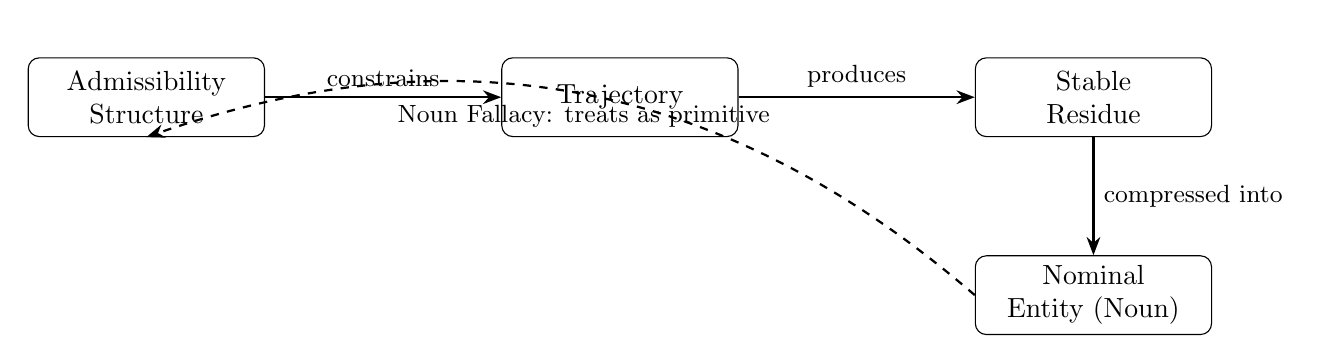
\begin{tikzpicture}[
  node distance=2cm,
  box/.style={rectangle, draw, rounded corners, minimum width=3cm, minimum height=1cm, align=center},
  arrow/.style={-{Stealth}, thick}
]
\node[box] (AS) {Admissibility\\Structure};
\node[box, right=3cm of AS] (TR) {Trajectory};
\node[box, right=3cm of TR] (SR) {Stable\\Residue};
\node[box, below=1.5cm of SR] (NE) {Nominal\\Entity (Noun)};

\draw[arrow] (AS) -- node[above, font=\small]{constrains} (TR);
\draw[arrow] (TR) -- node[above, font=\small]{produces} (SR);
\draw[arrow] (SR) -- node[right, font=\small]{compressed into} (NE);
\draw[arrow, dashed] (NE.west) to[bend right=30] node[below, font=\small]{Noun Fallacy: treats as primitive} (AS.south);
\end{tikzpicture}
\end{center}

The solid arrows represent the correct causal-explanatory order: the
admissibility structure constrains the possible trajectories; trajectories
produce stable residues when they dwell within bounded regions; stable
residues are compressed into nominal entities for cognitive economy.
The dashed arrow represents the Noun Fallacy: treating the nominal entity
as though it were more fundamental than the admissibility structure that
produced it.

\begin{principle}[Trajectory Compression Principle]
\label{prin:tcp}
Let $\mathcal{T} = (\omega_t, c_t)_{t \geq 0}$ be a trajectory in an
admissibility structure $(\Omega, \mathcal{C}, \{\to_c\})$. A noun $\mathbf{n}$
is an \emph{admissible compression} of $\mathcal{T}$ if it preserves
predictive utility over a specified neighborhood of the stable residue while
discarding trajectory information. The \emph{Noun Fallacy} occurs when
predictive utility is mistaken for ontological fundamentality: when the
fact that $\mathbf{n}$ correctly predicts local behavior is taken to imply
that $\mathbf{n}$ is a primitive of the theory rather than a compression of
the trajectory.
\end{principle}

Principle~\ref{prin:tcp} captures the central claim of this paper in a form
that is both mathematically precise and directly applicable to the cases
in Section~\ref{sec:survey}. The species name is an admissible compression
of an evolutionary trajectory: it predicts local reproductive and morphological
behavior reasonably well. It becomes the Noun Fallacy when the predictive
utility is taken to imply that species is a natural kind---a primitive with
an essential nature---rather than a compression of a lineage.

\subsection{Reachability as the Primary Relation}

\begin{observation}[Reachability Primacy]
\label{obs:primacy}
The Reachability Ontology of Principle~\ref{prin:reach-onto} implies that
the noun $\mathbf{n}$ is a useful compression precisely when $x$ is stably
reachable from a wide range of nearby configurations. It is a misleading
compression when reachability is inferred from past stability without
attending to whether the admissibility structure that produced that stability
is still operative. The stability of the noun is always inherited from the
stability of the admissibility structure; it is never intrinsic to the noun.
\end{observation}

The shift from existence to reachability as the primary relation changes what
counts as an explanation. To explain the existence of an entity is to derive
it from other entities. To explain the reachability of a configuration is to
describe the admissibility structure, trajectory dynamics, and relaxation
processes that make it accessible and stable. The explanatory target is richer,
and the questions that can be asked---about stability, disturbance, possible
change---are correspondingly expanded.

\subsection{Relaxation Dynamics and the Production of Residues}

The account of stable residues given so far has described their character---
regions of state space that trajectories inhabit for extended intervals---but
has not described how they are produced. The relevant process is
\emph{relaxation}: the dynamics by which a system under perturbation returns
toward a stable configuration, dissipating the tension introduced by the
perturbation.

Relaxation is not a single phenomenon. Different domains exhibit it under
different names and with different formal structures. In physics, it appears
as thermalization: a system initially far from equilibrium dissipates energy
into its environment until it settles into a thermal state. In ecology, it
appears as succession: a disturbed community of organisms moves through a
sequence of intermediate states toward a climax configuration. In cognitive
science, it appears as the resolution of cognitive dissonance or the
consolidation of memory: initially unstable representations relax toward
configurations that are coherent with the existing generative model. In
software engineering, it appears as the convergence of a distributed system
to a consistent state, or the settling of a codebase after a major refactor.

Despite their surface differences, these relaxation processes share a common
formal structure. There is an initial state $\omega_0$ that is perturbed
from the basin of attraction of some stable residue $x^*$. There is a
sequence of admissible transitions $\omega_0 \to_c \omega_1 \to_c \cdots
\to_c \omega_n \approx x^*$ that constitutes the relaxation trajectory.
There is a relaxation time $\tau$ that measures how long the process takes.
And there is a residual tension $\rho(\omega_t, x^*)$ that decreases
monotonically (under ideal conditions) as the trajectory approaches $x^*$.

\begin{definition}[Relaxation Trajectory]
A \emph{relaxation trajectory} from $\omega_0$ toward stable residue $x^*$
in admissibility structure $\mathcal{A}$ is a sequence
$\omega_0, \omega_1, \ldots, \omega_n$ of admissible transitions such that
$\rho(\omega_t, x^*)$ is non-increasing in $t$ and
$d_{\mathcal{A}}(\omega_n, x^*) < \epsilon$ for some convergence criterion
$\epsilon > 0$. The \emph{relaxation time} is $\tau = n$.
\end{definition}

Several features of relaxation dynamics are worth noting for the larger
argument.

First, relaxation is the mechanism that produces stable residues. A noun
earns its keep---acquires predictive utility---precisely when the relaxation
dynamics of the relevant domain reliably return perturbed configurations to
the same residue. The resilience of a species, the stability of an institution,
the robustness of a software module: all of these reflect the strength and
speed of the relevant relaxation dynamics, not intrinsic properties of the
entity named.

Second, relaxation can fail. When the admissibility structure shifts
sufficiently---when a constraint is introduced or removed that fundamentally
changes the basin geometry---the relaxation dynamics may no longer carry
the system toward the familiar residue. Instead of returning to $x^*$, the
trajectory may settle into a new residue $x^{**}$, or may fail to converge
at all, wandering through the state space without stabilizing. This failure
of relaxation is what produces the phase transitions in difficulty identified
in Section~\ref{sec:difficulty}: when the compiled abstractions that
constituted the familiar stable configuration are no longer valid, the system
cannot relax back to them.

Third, the \emph{rate} of relaxation encodes information about the depth of
the basin and the proximity of alternative attractors. Slow relaxation may
indicate a shallow basin (easily perturbed to another residue) or a high-dimensional
trajectory (many degrees of freedom must be coordinated before stability is
achieved). Fast relaxation indicates a deep basin or low-dimensional dynamics.
This is why mature expertise feels effortless and why learning new domains
feels effortful: mature expertise involves deep relaxation basins with short
relaxation times; new learning involves exploring a state space with no
pre-existing attractor structure, so every perturbation is slow to resolve.

\subsection{Specialized Realizations}

The general framework of admissibility structures, trajectories, and stable
residues is abstract enough to accommodate a wide range of specialized theories
across different domains. Three such realizations are worth noting: an RSVP
cosmological field theory in which material entities are stabilized admissibility
flows within an entropic potential field; a CLIO projection calculus in which
nominal entities are projections of higher-dimensional trajectory structures onto
lower-dimensional observational surfaces; and a Spherepop irreversible event
calculus in which computation proceeds by the collapse of reachability cones
through irreversible transitions. These are illustrative realizations of the
general framework, not its foundations. Appendix~\ref{app:realizations} works
through each in detail. Readers who find any particular realization unconvincing
are not thereby obliged to reject the general framework, which stands on the
independent evidence of the corrections surveyed in Section~\ref{sec:survey}.

%%%%%%%%%%%%%%%%%%%%%%%%%%%%%%%%%%%%%%%%%%%%%%%%%%%%%
\section{Possibility Versus Reachability}
\label{sec:possibility}
%%%%%%%%%%%%%%%%%%%%%%%%%%%%%%%%%%%%%%%%%%%%%%%%%%%%%

\epigraph{\textit{The existence of a solution is not equivalent to the
existence of a trajectory.}}{Notes}

\noindent
The Noun Fallacy obscures more than process. It also obscures possibility.
When a process is compressed into a static object, attention shifts toward
the properties of the present state and away from the structure of futures
that remain accessible from that state. A debt level, a city, a species,
a software system, or an institution appears as a thing possessing attributes
rather than as a position embedded within a landscape of admissible
trajectories.

This distinction gives rise to a fundamental asymmetry between possibility
and reachability. A state may exist within a possibility space while remaining
effectively unreachable from the current position. The existence of a solution
is therefore not equivalent to the existence of a trajectory toward it. Many
failures of analysis arise from conflating these notions. A reform may be
theoretically possible while remaining politically unreachable. A software
migration may be technically feasible while remaining organizationally
inaccessible. An ecological restoration may be biologically conceivable while
remaining practically unattainable given the current admissibility structure
and the cost of traversing the intermediate states.

The relevant question is not whether a future state exists, but whether an
admissible path to that state remains available from the current configuration.
A state can be clearly defined, carefully described, even mathematically
characterized, while being separated from the present by a sequence of
transitions that are inadmissible under current constraints. In the limit,
the state exists as a point in possibility space while being entirely
unreachable as a terminus of any admissible trajectory. The noun-centric
account, which represents both the current state and the target state as
entities with properties, cannot express this difference. It can describe
what is; it cannot describe what remains accessible from what is.

\subsection{Possibility Space and Trajectory Space}

We can formalize the distinction as follows. Given an admissibility structure
$(\Omega, \mathcal{C}, \{\to_c\})$, the \emph{possibility space} is simply
$\Omega$: all states that can in principle be described. The \emph{reachability
cone} from current state $x$ at time $t$ is $R_t(x) \subseteq \Omega$: all
states actually accessible by admissible transitions. The difference
$\Omega \setminus R_t(x)$ is the set of states that exist as possibilities
but are unreachable from $x$ under current conditions.

The possibility space is atemporal and context-independent: a state either
belongs to $\Omega$ or does not. The reachability cone is dynamic and
context-dependent: it evolves as the admissibility structure evolves and as
the current state changes. A process-primary account keeps both in view.
A noun-primary account collapses them together, treating whatever can be
described as thereby reachable.

\subsection{Convergence Without Reachability: A Recurring Failure Mode}

The confusion between possibility and reachability generates a characteristic
failure mode in planning, policy, and engineering: the specification of a
desired target state with detailed precision, without any account of the
trajectory constraints that determine whether that state is accessible.
The plan exists as a point in possibility space. Whether any admissible path
connects the current position to that point is a separate question that the
plan, as a noun-like entity, does not ask.

This failure mode appears so often across so many domains that it deserves
a name. We call it \emph{convergence without reachability}: the assumption
that because a target is well-specified, it is therefore approachable. Urban
renewal plans that describe desired neighborhood configurations without
attending to the displacement dynamics that their implementation would set
in motion. Software rewrites that specify a clean target architecture without
modeling the incremental transitions required to reach it from a legacy
codebase. Institutional reform proposals that describe ideal organizational
structures without tracing the political and procedural trajectories through
which current arrangements would need to be dissolved and reconstituted.

In each case, the plan treats the target as a noun---a stable entity with
desirable properties---while suppressing the trajectory question: is this
state reachable from here, by what sequence of admissible transitions, at
what cost? A process-primary planning framework asks the trajectory question
first. The target matters only insofar as it lies within the reachability
cone under realistic admissibility constraints. A beautiful target that lies
outside the cone is not a plan; it is a wish.

\subsection{Expanding the Reachability Cone as a Design Goal}

Once the distinction between possibility and reachability is explicit, a
new class of design goals becomes visible: not the specification of target
states but the expansion of the reachability cone. The goal is not to reach
any particular configuration but to increase the number of configurations
that remain accessible---to preserve and expand future options rather than
to optimize for any particular future.

This reframing has immediate practical consequences. A policy that achieves
a specific outcome while contracting the admissibility structure---eliminating
alternative approaches, foreclosing recovery paths, locking in dependencies
that cannot be undone---may be locally successful while globally harmful.
A policy that achieves a somewhat less optimal specific outcome while expanding
or maintaining the reachability cone may be locally suboptimal while globally
superior. Noun-centric evaluation cannot detect this difference because it
evaluates outcomes rather than trajectories. Reachability-centric evaluation
treats the health of the trajectory space as a primary criterion alongside
the quality of any particular outcome within it.

%%%%%%%%%%%%%%%%%%%%%%%%%%%%%%%%%%%%%%%%%%%%%%%%%%%%%
\section{The Geometry of Corrective Action}
\label{sec:geometry}
%%%%%%%%%%%%%%%%%%%%%%%%%%%%%%%%%%%%%%%%%%%%%%%%%%%%%

\epigraph{\textit{The practical difficulty of change depends less on the
magnitude of the desired outcome than on the geometry of the process
connecting current condition to target condition.}}{Notes}

\noindent
The tendency to reify processes into objects produces a corresponding tendency
to treat correction as a movement between states rather than as a navigation
of constraints. When viewed statically, a system appears to require only a
target condition: identify where the system should be, then move it there.
When viewed dynamically, the situation is more complex. Every corrective
action must traverse a landscape whose structure determines which
transformations are available, which are costly, and which are entirely
inaccessible from the current position.

\subsection{State Difference Versus Transformation Difficulty}

The geometric picture that process-primary theorizing supplies distinguishes
sharply between \emph{state difference} and \emph{transformation difficulty}.
Two states may be extremely similar---close together in any reasonable
metric on $\Omega$---while being separated by substantial barriers to
transition. A material that is one atom away from a stable crystal structure
may require enormous energy input to reach that structure from a disordered
phase. A legal system that needs only a single statute amended may require
decades of political realignment before the amendment becomes admissible.
A codebase that is architecturally close to a target design may be separated
from it by a sequence of intermediate refactoring steps each of which
introduces temporary instability that the production environment cannot tolerate.

Conversely, states that appear very different in their surface descriptions
may be connected by inexpensive trajectories. A political system that appears
to require fundamental restructuring may have a low-cost path to a better
outcome through a sequence of incremental adjustments each of which is
individually admissible under existing constraints. A software system that
appears to need a full rewrite may have a migration path through a series
of strangler-fig refactors that preserves functionality throughout.

The noun-centric account cannot express this distinction. It can measure the
distance between states; it cannot measure the cost of the trajectory between
them. The result is systematic misestimation of the difficulty of change:
large-seeming changes that traverse easy terrain are predicted to be hard;
small-seeming changes that require traversing constrained or barrier-laden
terrain are predicted to be easy.

\subsection{Bottlenecks, Corridors, and the Topology of Change}

A process-primary description of a change problem naturally focuses on the
topological features of the trajectory space: \emph{bottlenecks} (narrow
passages through which many trajectories must pass, making them fragile
under perturbation), \emph{corridors} (regions of relative ease connecting
separated parts of the state space), and \emph{barriers} (regions of
inadmissibility that separate otherwise accessible configurations).

\begin{definition}[Trajectory Bottleneck]
A state $b \in \Omega$ is a \emph{trajectory bottleneck} between regions
$A$ and $B$ if every admissible path from $A$ to $B$ passes through $b$,
or through a small neighborhood of $b$. The bottleneck is \emph{critical}
if its removal from the admissibility structure (i.e., making $b$ inadmissible)
disconnects $A$ from $B$ in the reachability relation.
\end{definition}

Critical bottlenecks are the points at which small changes to the
admissibility structure produce large changes to the reachability cone.
They are the locations of maximum leverage for both constructive and
destructive interventions: reachability can be expanded dramatically by
removing a barrier near a bottleneck, and contracted dramatically by
introducing a constraint that blocks one.

In urban planning, bottlenecks often appear as key parcels, infrastructure
nodes, or regulatory thresholds that determine whether particular development
trajectories are accessible. In software, they appear as the modules or
interfaces whose stability is required for all other components to function.
In institutional systems, they appear as the procedural steps, gatekeepers,
or information flows whose disruption would cascade into widespread
dysfunction. In all cases, the bottleneck is invisible to the noun-centric
account because it is a feature of the trajectory space, not a property of
any particular state.

\subsection{Corrective Action as Trajectory Design}

If correction is navigation of a trajectory space rather than movement
between states, then the design of corrective action requires trajectory
analysis rather than state specification. The relevant questions are:

\begin{enumerate}[leftmargin=*, label=(\roman*)]
\item What is the current position in the admissibility structure? Which
futures remain reachable from here?
\item Where are the bottlenecks on paths to desirable target regions?
Can they be widened, bypassed, or removed?
\item What intermediate states must be traversed, and are those intermediates
themselves stable enough to serve as way-points, or do they require sustained
costly effort to maintain while the next transition is prepared?
\item What perturbations during the transition could push the trajectory
into an undesirable basin, and how can those perturbations be anticipated
and buffered?
\item Does the corrective trajectory itself contract the admissibility
structure in ways that would limit future corrections---and if so, is that
acceptable?
\end{enumerate}

These questions are not answerable from a noun-centric description of the
problem. They require a process-primary account: an explicit model of the
admissibility structure, the reachability cone, and the cost landscape of
the trajectory space. The Admissibility Log of Section~\ref{sec:admlog}
is the natural recording architecture for this kind of analysis, since it
tracks precisely the changes to the admissibility structure that determine
which corrective trajectories are available.

%%%%%%%%%%%%%%%%%%%%%%%%%%%%%%%%%%%%%%%%%%%%%%%%%%%%%
\section{Hysteresis and Frozen Histories}
\label{sec:hysteresis}
%%%%%%%%%%%%%%%%%%%%%%%%%%%%%%%%%%%%%%%%%%%%%%%%%%%%%

\epigraph{\textit{The path back is not necessarily equivalent to the path
forward.}}{Notes}

\noindent
Processes frequently alter the conditions under which future processes occur.
A system that crosses a critical threshold often changes the structure of
its own future possibilities in ways that are not reversible by simply
retracing the path that produced the transition. Returning may require
substantially different actions---often far more costly ones---than those
that would have prevented the transition in the first place. This phenomenon
is \emph{hysteresis}: the dependence of future accessibility upon historical
trajectory.

Hysteresis is ubiquitous. It appears whenever a process modifies the
admissibility structure within which it operates. In physical chemistry,
a substance cooled below its freezing point and then reheated does not
pass back through the same sequence of states in the same direction: the
crystal structure formed during freezing imposes constraints on the melting
trajectory that were not present on the freezing trajectory. In ecology,
the removal of a keystone predator changes the trophic dynamics in ways
that cannot be reversed simply by reintroducing the predator; the ecosystem
has reorganized around the predator's absence, and the reintroduction faces
a different admissibility structure than the original system presented.
In software, a codebase that has accumulated years of technical debt cannot
be restored to an earlier clean state simply by reverting to an earlier
commit; the organizational knowledge, the external dependencies, and the
deployment infrastructure have all evolved around the current state.

\subsection{Hysteresis in the Admissibility Structure}

We can formalize hysteresis in the admissibility framework as follows.
Let $\mathcal{A}_0$ be the initial admissibility structure and
$\mathcal{A}_1$ be the structure after a transition event at time $t^*$.
The forward trajectory from $\mathcal{A}_0$ to $\mathcal{A}_1$ traversed
a sequence of intermediate structures. The question is: does there exist an
admissible trajectory from $\mathcal{A}_1$ back to $\mathcal{A}_0$?

If the transition event was \emph{admissibility-modifying}---if it changed
the transition relations themselves, not just the current state---then
the return trajectory must operate within $\mathcal{A}_1$, which may not
contain the transitions required to undo the changes. The transition may
have removed transitions from the admissibility structure that were required
for the return path. In that case, the system exhibits \emph{structural
hysteresis}: the admissibility structure itself is path-dependent, and the
return path, if it exists at all, is longer and more costly than the forward path.

\begin{definition}[Structural Hysteresis]
A transition from state $x$ to state $y$ via admissibility structure
$\mathcal{A}_0$ exhibits \emph{structural hysteresis} if the admissibility
structure after the transition, $\mathcal{A}_1$, has a strictly longer
minimum-cost path from $y$ back to $x$ than $\mathcal{A}_0$ had from $x$
to $y$. The \emph{hysteresis gap} is the difference in these path costs.
\end{definition}

Structural hysteresis is the formal correlate of what practitioners in many
domains call \emph{irreversibility}: not the absolute impossibility of
returning to a prior state, but the dramatic increase in cost that the
transition itself introduces into the return path.

\subsection{The Noun Fallacy and the Invisibility of Hysteresis}

The Noun Fallacy systematically obscures hysteresis because nouns suppress
the history through which the present state was reached. Two systems may
appear identical when described as objects with properties while possessing
radically different histories and therefore radically different futures. A
restored forest and a primary forest may have similar species compositions
while having entirely different soil microbiomes, mycorrhizal networks,
and structural complexity---and therefore entirely different admissibility
structures for future succession, disturbance response, and carbon dynamics.
A rebuilt institution and a never-disrupted institution may have similar
formal structures while having very different informal networks, tacit
knowledge distributions, and legitimacy reservoirs---and therefore very
different admissibility structures for future governance challenges.

A noun-centric account cannot detect this difference because the relevant
information is not contained within the current state. It is encoded in
the history of admissibility changes that produced the state: which
transitions were foreclosed during the disruption, which expertise was
lost, which relationships were severed, which options were eliminated.
The Admissibility Log recovers this information by recording the sequence
of $\Delta_t$ events rather than only the current state.

\subsection{Precautionary Principles as Hysteresis Recognition}

Many precautionary principles in ethics, law, and environmental policy
can be understood as institutionalized recognition of structural hysteresis.
The injunction to err on the side of caution when facing potentially
irreversible interventions is, in admissibility-theoretic terms, a rule
to prefer trajectories that maintain a large reachability cone over
trajectories that achieve near-term outcomes at the cost of structural
hysteresis. The precautionary principle does not prohibit action; it
weights the hysteresis gap as a significant cost that should enter the
analysis of any intervention.

What is often missing from precautionary reasoning is a formal account of
how to measure the hysteresis gap---how to estimate the increased cost of
the return path that an intervention would introduce. Process-primary theorizing
provides the framework for such measurement: it requires modeling the
admissibility structure before and after the proposed intervention and
estimating the difference in return-path costs. This is not always possible
in practice, given the complexity of real-world admissibility structures.
But the framework at least makes clear what the relevant question is and
why purely outcome-based evaluation systematically underweights it.

%%%%%%%%%%%%%%%%%%%%%%%%%%%%%%%%%%%%%%%%%%%%%%%%%%%%%
\section{Reachability as an Ontological Primitive}
\label{sec:ontprim}
%%%%%%%%%%%%%%%%%%%%%%%%%%%%%%%%%%%%%%%%%%%%%%%%%%%%%

\epigraph{\textit{Persistence is not fundamental. Persistence is a special
case of stable reachability.}}{Notes}

\noindent
The preceding sections have developed reachability as a useful analytical
concept. This section argues for a stronger claim: that reachability is an
\emph{ontological} primitive, more fundamental than existence in the
conventional sense, and that the apparent priority of existence over
reachability is itself an artifact of the Noun Fallacy applied to ontology.

\subsection{Reversing the Conventional Order}

Traditional ontology begins with objects and asks what processes connect
them. Process-primary ontology reverses this order. It begins with
trajectories and asks which apparent objects emerge as stable regions within
a larger flow. The reversal is not merely methodological---it is not just
a different way of describing the same underlying reality. It is a claim
about which level of description is more fundamental.

The argument for reversal runs as follows. Every object we encounter---every
apparently stable entity whose persistence we take for granted---is stable
because there is an ongoing process sustaining it. Remove the process and the
object dissolves. The process is therefore not dependent on the object;
the object is dependent on the process. The fundamental level is the
process level. Objects are the appearance that processes present to
observation at certain scales.

This is not idealism, and it is not the claim that objects are illusions.
It is the claim that when we explain why an object persists, the explanation
must bottom out in process terms---in the dynamics that produce and sustain
the stable configuration---rather than in object terms. Explaining persistence
by reference to the object's intrinsic properties is always either circular
(the object persists because it has the property of persisting) or deferred
(the intrinsic properties are themselves sustained by processes not yet
examined).

\subsection{Persistence as Stable Reachability}

The positive formulation is: \emph{persistence is a special case of stable
reachability}. An object persists over an interval $[t_0, t_1]$ if and only
if, for every $t \in [t_0, t_1]$, the state $x$ that the object occupies
is stably reachable from the states it occupied in $[t_0, t]$. Persistence
is not a brute fact about the object; it is a derived fact about the
trajectory and the admissibility structure within which the trajectory moves.

This reformulation has several immediate consequences.

First, it explains why the same kind of entity can persist in some
environments and not others. A species persists in an environment where
the admissibility structure supports the reproductive and ecological dynamics
that constitute its existence. It fails to persist in an environment where
those dynamics are no longer admissible---where habitat loss, invasive
species, or climate change have removed the transitions required for the
lineage to continue. The persistence of the species is not a property of
the species; it is a property of the relationship between the species and
its admissibility structure.

Second, it explains why apparent stability can be deceptive. A system may
exhibit stable persistence over an interval while its admissibility structure
is contracting---while the reachability cone is narrowing around the current
trajectory and the space of available futures is shrinking. The object
appears stable because it is still following its trajectory; but the
trajectory is heading toward a region from which return and adaptation will
be very costly. The noun-centric account detects current stability; the
reachability-centric account detects structural fragility.

Third, it dissolves certain persistent puzzles in philosophy of identity.
The ship of Theseus puzzle asks whether an object that has had all its
parts replaced is the same object. The process-primary answer is that the
question is malformed: what matters is not whether the current material
constituents are the same but whether the trajectory of the system exhibits
continuity with the prior trajectory in the relevant admissibility structure.
If the replacement process preserved the functional relations, the navigation
history, and the social role of the ship---if the trajectory through the
relevant admissibility structure was continuous---then it is the same ship
in the sense that matters. If the replacements disrupted these relational
continuities, it is not, regardless of how many planks remained.

\subsection{Objects as Compressed Trajectory Summaries}

The ontological reformulation gives a precise account of what objects are:
they are \emph{compressed summaries of trajectory structure}. A noun does
not name a thing that has properties independent of any process. It names
a region of the admissibility structure within which many trajectories
converge on compatible descriptions. The convergence---the fact that many
different starting points and many different historical paths produce
similar current descriptions---is what gives the noun its apparent
referential solidity.

\begin{principle}[Ontological Compression]
\label{prin:onto-compress}
A nominal entity $\mathbf{n}$ is an \emph{ontologically legitimate
compression} if and only if there exists an admissibility structure
$\mathcal{A}$ and a basin of attraction $\mathcal{B}(x^*)$ such that
(a) the trajectories compressed under $\mathbf{n}$ all pass through
$\mathcal{B}(x^*)$, (b) the basin is stable under the admissibility
dynamics of $\mathcal{A}$, and (c) the compression discards no information
required for predicting how $\mathbf{n}$-labeled trajectories will respond
to perturbations relevant to the purposes of the theory.

The Noun Fallacy consists in using a compression that fails condition (c):
that discards trajectory information required for accurate prediction of
responses to perturbation, stability analysis, or recovery planning.
\end{principle}

Principle~\ref{prin:onto-compress} makes precise what it means for a noun
to be ``legitimate'' while remaining incomplete. All nouns discard information;
the question is whether they discard information that matters for the purposes
at hand. The Noun Fallacy is not the use of nouns but the use of nouns that
discard relevant trajectory information while treating the noun as though it
were a complete description.

\subsection{The Consequences for Theory Construction}

If reachability is ontologically primary, then the construction of theories
should begin with the admissibility structure and derive the nominal entities
as its stable configurations, rather than beginning with nominal entities and
asking what relations hold among them. This is a methodological prescription
with practical consequences for how theories in any domain are built and
evaluated.

A theory that begins with admissibility structures will naturally include
accounts of how its central entities come to exist (which trajectories
produce them), why they persist (which admissibility dynamics sustain the
basin), and how they change or dissolve (which perturbations push trajectories
out of the basin). A theory that begins with nominal entities can add these
accounts later, but only by introducing a separate dynamics that was not part
of the original framework---and the subsequent integration is often awkward
precisely because the original nominal primitives do not have the right
properties for the dynamics to attach to cleanly.

The independent corrections surveyed in Section~\ref{sec:survey} can all
be read as cases where the noun-first strategy reached its limits and was
forced to introduce trajectory dynamics as an afterthought---and where the
introduction proved so productive that it eventually reorganized the entire
theoretical framework around the dynamics, demoting the original nominal
primitives to the status of derived, contextually useful compressions.

%%%%%%%%%%%%%%%%%%%%%%%%%%%%%%%%%%%%%%%%%%%%%%%%%%%%%
\section{Re-Nominalization: How Process Insights Are Converted Back}
\label{sec:renominalization}
%%%%%%%%%%%%%%%%%%%%%%%%%%%%%%%%%%%%%%%%%%%%%%%%%%%%%

\epigraph{\textit{The software community took Alexander's transformation
language and converted it back into forms.}}{Conversation notes}

\noindent
The preceding sections have established that the Noun Fallacy is repeatedly
corrected across domains and that the corrections share a common structure.
This section examines the inverse phenomenon: the conversion of a process
insight back into a nominal entity under institutional and paradigmatic
pressure. The software industry's reception of Christopher Alexander's work
provides a uniquely instructive case because the re-nominalization is
historically documented and structurally unambiguous.

\subsection{Alexander's Progressive Process Recovery}

Alexander's career exhibits a clear trajectory from nominal to process
accounts. His 1964 dissertation \citep{alexander1964} proposed that design
problems should be decomposed into networks of interacting requirements,
connected by positive and negative relations. The vacuum cleaner example---
his test case---was not represented as a collection of components but as a
signed graph of forces: performance, simplicity, economy, and jointing,
connected by mutual compatibility and incompatibility relations. The design
problem was to find a configuration that minimized the total tension in the
graph.

This is not object arrangement. It is constraint satisfaction over a network
of interacting forces. The solution is not a thing but a configuration---a
stable point in a space of possible arrangements, reached by a process of
tension reduction. The vacuum cleaner form that results is the residue of a
process of constraint negotiation; it does not exist independently of the
forces that generate it. In the language of Section~\ref{sec:framework}:
the force graph is the admissibility structure, the design process is the
trajectory, and the final form is the stable residue.

\emph{A Pattern Language} \citep{alexander1977} sharpened this analysis.
Patterns were described not as reusable object structures but as
transformation rules, taking the form:

\begin{center}
\textbf{Context} $+$ \textbf{Forces} $\longrightarrow$ \textbf{Configuration}
\end{center}

The pattern was a process description. Its validity was contextual and
dynamic---dependent on the forces being present, not derivable from the
pattern's structure in isolation from its field of application.

\emph{The Nature of Order} \citep{alexander2002} carried this trajectory
to its limit. Centers---Alexander's fundamental unit of living structure---
are not objects. They are regions of intensified field coherence: zones in
which structural dynamics conspire to sustain a local organization. A center
exists because surrounding structure reinforces it; it persists because field
dynamics support it; it dissolves when those dynamics shift. This is a field
description, not an object description. The fifteen fundamental properties
Alexander identifies are all relational: they describe how one region of
structure mediates force across another, not how isolated objects behave.

Alexander spent forty years moving the explanatory burden progressively
upstream, from the form (the residue) toward the forces (the admissibility
structure) that generate it. The frustration visible in his later work---his
repeated insistence that architects and software engineers were missing the
point---reflects the frustration of someone who had reached a process-primary
account but lacked the formal language to make the admissibility structure
explicit. The Nature of Order's qualitative descriptions of centers and
living structure are gesturing at something like relaxation dynamics and
stability wells, but without the mathematics to pin it down.

\subsection{The Gang of Four Inversion}

The Gang of Four design patterns \citep{gamma1994} introduced the notion
of a software design pattern by explicit reference to Alexander's work.
The reference was sincere and the intellectual debt genuine. But the
translation was structurally inverted.

Alexander's patterns, as argued above, were transformation rules: context
plus forces yields configuration. The pattern was a description of a process
of tension resolution. The Gang of Four patterns are object structures:
a Visitor is a class hierarchy with a particular interface arrangement; a
Singleton is a class with a private constructor and a static instance
accessor; a Factory is a class that encapsulates object creation. Each
pattern is a noun-form---a reusable entity structure---not a transformation
rule.

\begin{table}[h]
\centering
\caption{The structural inversion: Alexander's framework versus its software reception}
\begin{tabular}{p{0.44\textwidth} p{0.44\textwidth}}
\toprule
\textbf{Alexander's Framework} & \textbf{Gang of Four Interpretation} \\
\midrule
Pattern as transformation rule & Pattern as reusable entity structure \\
Context $+$ forces $\to$ configuration & Template instantiated in context \\
Design as constraint negotiation & Design as entity arrangement \\
Solution is a stabilized trajectory & Solution is a static configuration \\
Form is the residue of forces & Form is the specification of parts \\
Patterns are context-sensitive resolutions & Patterns are portable structures \\
\bottomrule
\end{tabular}
\label{tab:alexander}
\end{table}

The inversion illustrates something important about the Noun Fallacy's
persistence: even when a theorist is explicitly working toward a
process-primary account, the institutional and paradigmatic pressures of
the receiving field can reverse the direction of travel. Alexander was
trying to dissolve the noun; software engineering received the work and
reconstituted a noun from it. The re-nominalization was not malicious or
careless. It was the natural consequence of fitting a process insight into
an entity-organized toolkit---of mapping Alexander's word ``pattern'' onto
the conceptual resources available in the dominant computational paradigm
of the time.

\subsection{The Structural Logic of Re-Nominalization}

The Alexander case is instructive not just as a historical curiosity but as
an illustration of the structural logic by which re-nominalization proceeds.
It follows a recognizable pattern:

\begin{enumerate}[leftmargin=*, label=(\arabic*)]
\item A theorist working within a noun-primary framework encounters phenomena
that resist nominal treatment. The nominal primitives prove insufficient.

\item The theorist begins recovering the process: forces, trajectories,
constraint fields, transformation rules.

\item The recovery is communicated in a form accessible to a broader
community. The communication necessarily uses the available vocabulary
of the receiving field.

\item The receiving field maps the communicated content onto its existing
conceptual apparatus. Transformation rules are read as object structures.
Force fields are read as attribute sets. Trajectories are read as sequences
of states.

\item The re-nominalized version circulates and becomes the canonical
interpretation. The process content is preserved only in the original texts,
which are now read through the lens of the re-nominalized interpretation.
\end{enumerate}

This logic explains why the correction of the Noun Fallacy does not proceed
smoothly once a process-primary account has been achieved. The account must
be communicated; communication occurs in the vocabulary of the receiving
field; and that vocabulary shapes what can be heard. The formal framework
developed in Section~\ref{sec:framework}---admissibility structures,
trajectories, stable residues---is an attempt to provide a vocabulary that
resists re-nominalization by making the process structure explicit in its
very terms.

%%%%%%%%%%%%%%%%%%%%%%%%%%%%%%%%%%%%%%%%%%%%%%%%%%%%%
\section{Difficulty as a Relational Property}
\label{sec:difficulty}
%%%%%%%%%%%%%%%%%%%%%%%%%%%%%%%%%%%%%%%%%%%%%%%%%%%%%

\epigraph{\textit{Difficulty is not a noun but a relation.}}{Flyxion,
\emph{Noun-Free Cognition}, 2026}

\noindent
The Noun Fallacy is not confined to scientific theory. It operates with
particular force in cognitive science and artificial intelligence, where
it shapes not only theoretical frameworks but practical assessments of
what systems can and cannot do. In this domain, the entity most
insistently treated as a noun is \emph{difficulty} itself---the apparent
property of a task that determines how much cognitive or computational
effort it requires.

Difficulty is one of the most frequently reified quantities in cognitive
science and AI. We speak of a task being difficult as though difficulty
were an intrinsic property of the task, rather than a relation between
a task, a system, a compilation state, and an environment. That reification
is a direct instance of the Noun Fallacy, and it generates the same failure
mode: systematic prediction error whenever the relational structure that
constitutes the difficulty changes.

\subsection{The Standard View and Its Failure}

The standard view treats difficulty as intrinsic to tasks.
On this view, intelligence is a capacity that gradually expands to encompass
harder and harder problems, and the trajectory of technological or cognitive
development is a progressive conquest of the difficult by the capable.

This view generates persistent prediction failures. Tasks declared permanently
resistant to automation are abruptly rendered trivial. Tasks assumed to be
straightforward prove stubbornly intractable \citep{moravec1988,autor2015}.
Chess provides the canonical illustration. For much of the twentieth century,
mastery of chess functioned as a proxy for strategic intelligence. The defeat
of human champions by specialized machines was initially interpreted as the
conquest of a hard cognitive problem. But within a short period, chess ceased
to function as a meaningful benchmark---not because it became easier in any
absolute sense, but because the scaffolding that constituted its difficulty
as a cognitive measure dissolved. What changed was not the game but the
compilation state available to machines.

\subsection{Relational Difficulty: Formal Account}

Difficulty is formally a function of at least four variables: the task
specification $T$, the system $S$ attempting it, the set of compiled
affordances $\mathcal{P}$ available to $S$, and the environment $E$ in
which execution occurs:

$$D: (T, S, \mathcal{P}, E) \longrightarrow \mathbb{R}^+$$

where $\mathbb{R}^+$ denotes the non-negative reals. Crucially, $D$ is not
invariant under transformations of $\mathcal{P}$ or $E$ even when $T$ and
$S$ are held fixed. Small perturbations to $\mathcal{P}$---the introduction
of a new tool, abstraction, or precompiled structure---can produce
discontinuous changes in $D$.

\begin{theorem}[Non-Intrinsicness of Difficulty]
\label{thm:difficulty}
For any task $T$ and system $S$, there exist compilation states $\mathcal{P}_1$,
$\mathcal{P}_2$ and environments $E_1$, $E_2$ such that
$$D(T, S, \mathcal{P}_1, E_1) \gg D(T, S, \mathcal{P}_2, E_2).$$
Therefore no context-free difficulty measure exists for any non-trivial
class of tasks.
\end{theorem}

In the language of the general framework, the compilation state $\mathcal{P}$
is a component of the admissibility structure: it determines which transitions
between problem states are available to the system. The difficulty $D$ is a
measure of path length in the reachability relation: how many steps are
required, in the current admissibility structure, to reach a solution from
the current state. A new tool or abstraction changes the admissibility
structure and thereby changes all path lengths, potentially collapsing a
long path into a short one and making a previously hard task trivially easy.

\subsection{Empirical Instantiation: Neural Manifolds and the Geometry of Difficulty}

Theorem~\ref{thm:difficulty} is a formal result, but it has direct
experimental support from recent neuroscience. The BCI learning study
described in Section~\ref{sec:survey} \citep{busch2026} provides a
controlled empirical demonstration of non-intrinsic difficulty at the
level of individual neural geometry.

Recall that participants were trained on three types of BCI control
mapping: an intuitive mapping aligned with the dominant direction of
their intrinsic neural manifold, a within-manifold perturbation requiring
activity along a secondary manifold direction, and an outside-manifold
perturbation requiring activity patterns that fell outside the manifold
entirely. The three mappings were formally equivalent as control tasks:
in each case the participant needed to generate a brain activity pattern
that steered an avatar toward a goal. What differed was the geometric
relationship between the target mapping and the participant's current
admissibility structure.

The gradient of learnability---fast, slow, impossible---directly measures
what Theorem~\ref{thm:difficulty} predicts. Holding the task $T$ fixed
and the system $S$ fixed, variation in the compilation state $\mathcal{P}$
(here: the geometric relationship between the target and the current
neural manifold) produces dramatic variation in $D$. The intuitive mapping
is easy not because it is intrinsically simple but because it lies within
the high-variance region of the reachability cone. The outside-manifold
mapping is not merely harder; it is effectively unreachable within
the training period available, instantiating the $D \to \infty$ limit
of the non-intrinsicness theorem.

The study also operationalizes the distinction between
possibility and reachability at neural resolution. The outside-manifold
states are genuinely possible: participants' neurons are capable in
principle of generating those activity patterns. The study verified that
both within- and outside-manifold components produced decodable movement
patterns, confirming that the neural signals were present. Yet the
outside-manifold states were not reachable within the available learning
horizon, because no sequence of admissible transitions from the current
neural state led to the required pattern efficiently. Possibility and
reachability come apart precisely, in a controlled laboratory setting,
at the boundary of the intrinsic manifold.

\subsubsection*{Implications for AI Benchmarking}

The BCI finding has direct implications for the evaluation of artificial
intelligence systems, which is a major locus of the Noun Fallacy in
contemporary practice. AI benchmarks are typically constructed by
specifying target tasks and measuring performance---treating difficulty
as a property of the task and capability as a property of the system.
The BCI results suggest a different picture.

What determines whether an AI system can learn a task is not primarily
the structure of the task but the geometric relationship between the
task and the system's current admissibility structure---its ``intrinsic
manifold'' of easily activatable computational patterns, shaped by prior
training. A task that is formally simple but geometrically distant from
the system's current distribution is harder than a formally complex task
that lies within the natural variance of the system's activity.

This implies that benchmark scores cannot be interpreted as measuring
intrinsic task difficulty or intrinsic system capability. They measure
a relational quantity: the alignment between the task's demands and
the system's current admissibility structure. The same task will receive
different scores from systems with different training histories, not
because of differences in raw capability but because of differences in
the geometry of their learned manifolds. Benchmark comparisons between
systems with different training distributions are therefore structurally
analogous to comparing BCI learning rates between participants with
different intrinsic neural manifolds: the comparison is valid only if
the admissibility structures are held constant, which they typically
are not.

Abstraction, on the process-primary account, is not the discarding of detail
to reveal underlying structure. It is the compilation of prior resolved
structure into a callable interface: a transition in the admissibility
structure that replaces a complex chain of steps with a single admissible
operation.

The compilation is always against a target environment. A proved theorem can
be invoked as a lemma without reproving it---but only as long as the logical
framework within which it was proved remains operative. A driving skill, once
compiled, operates without conscious attention to the mechanics of clutch and
steering---but only as long as the interface between driver and vehicle remains
within the envelope in which the skill was compiled. Every abstraction embeds
assumptions about the stability of its compilation environment.

\begin{principle}[Compilation Instability]
\label{prop:instability}
For any abstraction $a$ compiled against environment $E_0$, there exists
a sequence of environmental changes $E_0, E_1, \ldots, E_n$ such that
$\sigma(a, E_n) < \theta$: any compiled abstraction eventually becomes
brittle under some environmental trajectory.
\end{principle}

Proposition~\ref{prop:instability} follows from the open-ended nature of
environments. Environments are not closed systems; they are continually
reshaped by the very abstractions deployed within them. This reflexivity is
not a design flaw but a structural feature of adaptive systems operating in
co-evolving environments.

\subsection{Goodhart Dynamics as Re-Nominalization}

The mechanism by which successful process descriptions are converted back
into nominal entities is analyzed with particular precision under the rubric
of Goodhart's Law: when a measure becomes a target, it ceases to be a good
measure \citep{goodhart1984,strathern1997}.

In the framework of this paper, Goodhart dynamics are a special case of
re-nominalization. A process is observed; it is compressed into a metric
that captures some of its relevant features; the metric is adopted as a
target; optimization pressure selects for states that score well on the
metric without necessarily preserving the process that made those states
worth scoring. The metric---the noun---is treated as the real thing, and
the process it was compressing is no longer visible.

\begin{example}[Goodhart Dynamics as Noun Fallacy]
Research evaluation adopts citation counts as a proxy for research quality.
The proxy is initially useful: citation counts encode, in compressed form,
something about the distribution of engagement across the research community.
As a target, citation counts attract optimization pressure that operates on
the metric rather than the underlying process. Strategic citation networks,
salami slicing, and fashionable conformity optimize the compressed label
without preserving the dynamics that made the label informative. The noun
``high-citation research'' has been severed from the process
``influential research''; the former is optimized; the latter degrades.
\end{example}

Goodhart dynamics are therefore the expected consequence of treating any
relational property as intrinsic. Once a property has been nominalized---given
a label treated as naming something stable and measurable independently of
context---it becomes a target for optimization that operates on the label
rather than the underlying process. The dynamics that generated the
labeling-worthy behavior are invisible to the optimizer; only the label
is visible. The Noun Fallacy, in this domain, is not merely a theoretical
error but an active mechanism of institutional and technological degradation.

%%%%%%%%%%%%%%%%%%%%%%%%%%%%%%%%%%%%%%%%%%%%%%%%%%%%%
\section{The Politics of Nominalization: Power, Visibility, and Contested Residues}
\label{sec:politics}
%%%%%%%%%%%%%%%%%%%%%%%%%%%%%%%%%%%%%%%%%%%%%%%%%%%%%

\epigraph{\textit{All reification is a forgetting.}}{Theodor Adorno,
\textit{Minima Moralia}}

\noindent
The Noun Fallacy has so far been treated primarily as an epistemic and
methodological error: the mistake of treating a compressed residue as a
foundational entity. But nominalization is never only epistemic. The choice
of which processes to compress into nouns, and which nouns to treat as
foundational, is always also a political choice. It distributes visibility
and invisibility, legitimacy and illegitimacy, across social and material
processes. This section examines the political dimension of nominalization
and its correction.

\subsection{Who Benefits from Which Nouns}

Every nominalization distributes costs and benefits asymmetrically. When a
corporation is treated as a legal person---a nominal entity with rights and
standing---the processes that constitute it (the labor of its workers, the
externalization of its environmental costs, the contingency of its contractual
arrangements) are rendered legally invisible. The corporation as noun can hold
property, enter contracts, and bear liability, while the processes that sustain
it can be reorganized, relocated, or dissolved in ways that the nominal entity
absorbs without legal consequence. The nominalization serves interests: it
enables capital to organize itself in ways that would be impossible if the
underlying processes were legally legible.

The species concept, nominalized into a legal category for conservation law,
distributes benefits to those who work within taxonomic frameworks and costs
to those whose activities are constrained by species listings---while
rendering invisible the habitat processes, trophic dynamics, and dispersal
mechanisms that actually determine whether a population persists. A population
can be legally protected while being functionally eliminated if the nominalized
category fails to track the relevant processes.

The pattern is general. Nominalizations concentrate visibility on the residue
and distribute invisibility to the trajectory. The residue is legible to
institutions; the trajectory is not. Those whose interests are served by
the residue benefit from this distribution; those whose interests are served
by the trajectory do not. The Noun Fallacy is therefore not merely a cognitive
default but a tool of governance that can be deployed, maintained, and defended
against process-primary analysis.

\subsection{Contested Residues and Process Recovery as Political Act}

When a nominalization is contested---when some parties insist that the noun
names something real and others insist that the noun is a misleading compression
of a process that needs to be recovered---the dispute is often described as
a technical or scientific disagreement. It is also a political one.

The debate over whether ``race'' names a biological reality or a social
process is a paradigmatic case. Those who maintain the nominalization argue
that race names a stable, heritable category. Those who recover the process
argue that race is a socially produced trajectory through a space of
classification practices, power relations, and material conditions---a
trajectory that is real and consequential but that is not well described by
the nominal entity it has been compressed into. The stakes of the dispute
are not merely taxonomic: they determine what kinds of interventions are
admissible, what kinds of harm are legible, and what kinds of repair are
possible.

Similar dynamics appear in the nominalization of ``disability'' (a stable
property of individuals, or a mismatch between individual trajectories and
an admissibility structure that could be changed?), ``poverty'' (a condition
of persons, or a feature of the admissibility structure that determines
which economic trajectories are accessible?), and ``merit'' (an intrinsic
property of individuals, or a compression of a trajectory through a space
of differentially accessible preparation, assessment, and certification?).

In each case, process recovery is not merely an epistemic improvement but
a political reorientation: it shifts the question from ``how do we manage
people with this property?'' to ``what admissibility structure produces this
apparent property, and what would it take to change that structure?'' The
process-primary question is systematically harder for existing institutions
to answer, because it requires acknowledging that the institution's own
operations are part of the admissibility structure being described.

\subsection{The Visibility of Labor and the Invisibility of Infrastructure}

One of the most consequential effects of nominalization at scale is the
systematic invisibility of maintenance, care, and infrastructure labor. The
nominal entities that societies produce and consume---buildings, software
systems, institutions, cultural artifacts---are highly visible. The ongoing
labor that sustains them---cleaning, debugging, updating, repairing,
regulating, caring---is structurally invisible to the noun-centric account
because it is the process that keeps the residue stable, not the residue
itself.

This invisibility is not accidental. A process-primary account of a software
system would assign prominence to the maintenance engineers who keep it
running, the operations staff who manage its infrastructure, and the support
workers who handle its edge cases---because these are the people sustaining
the admissibility structure within which the system operates as a stable
nominal entity. The noun-centric account assigns prominence to the authors
of the original code, because that is the act that produced the residue.
The nominal entity is attributed to its origin, not to its maintenance; the
trajectory is invisible; the labor of ongoing process sustenance goes
unrecognized and undercompensated.

This is the Noun Fallacy as a theory of labor value. It systematically
undervalues work that sustains trajectories in favor of work that produces
residues, because the residue is visible and the trajectory is not. A
process-primary political economy would recognize sustaining work as
constitutive rather than ancillary---not maintaining something that already
exists but continuously producing the conditions under which the nominal
entity remains stably reachable.

\subsection{Process Recovery as Institutional Reform}

If nominalizations distribute visibility and invisibility, power and
powerlessness, then process recovery---the systematic project of asking what
trajectories nouns compress---is not merely a methodological discipline
but an institutional one. It requires building institutions that can see,
record, and govern trajectories rather than only nominal entities.

The Admissibility Log, developed in Section~\ref{sec:admlog}, is one such
institutional form. An institution that tracks changes to its admissibility
structure---what became possible, what became impossible, who gained options
and who lost them---is an institution that cannot easily hide its political
choices behind nominal entities. Every constraint introduced or removed is
a first-class record. Every reachability contraction is legible. The political
choice of which trajectories to sustain and which to allow to dissolve is
not hidden behind the apparent stability of the resulting noun.

This does not make the Admissibility Log politically neutral. It makes it
politically transparent. The choice of which admissibility changes to record,
which to prioritize, and which baseline to set for reachability volume is
itself a political choice. Process-primary institutions do not eliminate
politics; they relocate it from the invisibility of unstated nominal
assumptions to the legibility of contested admissibility decisions.

%%%%%%%%%%%%%%%%%%%%%%%%%%%%%%%%%%%%%%%%%%%%%%%%%%%%%
\section{Process-Primary Theorizing Without Reifying Process}
\label{sec:method}
%%%%%%%%%%%%%%%%%%%%%%%%%%%%%%%%%%%%%%%%%%%%%%%%%%%%%

\epigraph{\textit{What is needed is not a commitment to process as a
metaphysical primitive but a sustained methodological discipline.}}{Conversation notes}

\noindent
The argument of this paper must confront a symmetric danger. Having diagnosed
the Noun Fallacy and traced its operations across multiple domains, it would
be easy to fall into the symmetric error: to reify ``process'' as a new
fundamental substance, to treat the transition from entity-thinking to
process-thinking as a final discovery, or to claim that any particular formal
framework provides the unique substrate beneath all the corrections surveyed.

\subsection{Process Is Not a Privileged Primitive}

The argument of this paper is not that processes are more real than entities.
It is that entities, as treated in theoretical practice, are often compressed
descriptions of processes---and that the compression should be acknowledged
rather than forgotten. The corrective move is not to substitute ``process''
for ``entity'' as the foundational primitive. It is to ask, for any putative
primitive, what trajectory it compresses and what admissibility structure
sustains it.

This is the point that distinguishes the present framework from process
philosophy in the tradition of Whitehead \citep{whitehead1929} and from
process-theoretic approaches in cognitive linguistics \citep{langacker1987}.
Those traditions replace entities with processes, but they typically treat
processes as the new foundational substance---a different kind of thing,
but still a thing. The resulting metaphysics faces the same structural
problem as entity-based metaphysics: asked what the process is, the answer
is either circular or infinitely regressive.

The move proposed here is different. It is not metaphysical but methodological:
a discipline of always asking about the trajectory that a nominal entity
compresses, without assuming that the trajectory is itself a primitive.
The trajectory is an abstraction too, and it encodes assumptions about what
counts as a state, a transition, and an admissible transformation. Those
assumptions may themselves need to be examined.

This also explains why the formal frameworks in Section~\ref{sec:framework}---
admissibility structures, RSVP, CLIO, Spherepop---are presented as scaffolds
rather than foundations. A scaffold is erected to enable construction under
conditions where direct access is impossible or unsafe. Once the structure
it supports is complete, the scaffold becomes not merely unnecessary but
obstructive. Conceptual, mathematical, and linguistic scaffolds serve their
purpose only insofar as they remain provisional. The value lies in what they
make possible, not in their preservation.

\subsection{The Four Methodological Questions}

What remains after the formalisms are demoted from primitive to scaffold
status is a methodological discipline. It consists in a set of questions
that a process-primary theorist asks about any proposed explanatory primitive:

\begin{enumerate}[leftmargin=*, label=(\roman*)]
\item \textbf{Trajectory recovery.} What trajectory does this primitive compress?
That is, what sequence of states and transitions, in what admissibility
structure, produced and sustains the configuration named by this primitive?

\item \textbf{Stability analysis.} What stability condition does this primitive
satisfy? What is the stability functional $\sigma(a, E)$ for this abstraction,
and what environmental changes would push it below threshold?

\item \textbf{Foreclosure audit.} What is foreclosed by treating this as
primitive? What questions---about origin, stability, variation, dissolution---
become invisible when the trajectory is compressed into the nominal entity?

\item \textbf{Re-nominalization pressure.} What institutional, technological,
or paradigmatic forces are likely to convert any process description derived
from this inquiry back into a nominal entity?
\end{enumerate}

These questions do not have universal answers. They are context-specific
and domain-relative. But the discipline of asking them---consistently,
across domains, and with respect to one's own theoretical commitments
as much as those of others---is what process-primary theorizing consists in.

\subsection{Wittgenstein and the Anti-Essentialist Lineage}

The discipline described above has a philosophical lineage in the later work
of Wittgenstein \citep{wittgenstein1953}. Wittgenstein's refusal to define
language games or family resemblances was a methodological commitment:
definitions aim to fix meaning by specifying necessary and sufficient
conditions, but meaning is inseparable from use, and use shifts across
contexts in ways that no definition can track in advance.

The present framework extends this commitment from semantics to ontology.
What Wittgenstein showed for words---that their apparent stability is a byproduct
of temporarily successful coordination---the argument here extends to
theoretical primitives in general. Treating them as having fixed,
context-independent natures forecloses exactly the questions that inquiry
needs to ask.

The extension beyond Wittgenstein lies in a shift from semantics to action:
not only can the meaning of a word not be fixed by definition, but the
difficulty of a task cannot be fixed by analysis. Both are products of living
systems that stabilize patterns temporarily and then move on. The impossibility
of predicting task difficulty is not an epistemic limitation to be overcome but
a structural consequence of taking anti-essentialism seriously at the level of
cognitive and computational ontology.

\subsection{The Positive Program: Designing for Reachability}

The preceding three subsections are largely negative: they identify what
process-primary theorizing refuses (entity metaphysics, process metaphysics,
the illusion of finality) and how it relates to prior anti-essentialist
work. This subsection states the positive program.

Process-primary theorizing, when it moves from critique to construction,
asks a single organizing question: \emph{how do we design systems, theories,
and institutions that sustain reachability rather than merely producing
residues?} This question has answers at multiple levels.

At the level of \textbf{theoretical design}, process-primary theorizing
recommends choosing primitives that encode admissibility structures and
trajectories rather than nominal entities. A theory of learning that takes
``knowledge'' as primitive will build in the Noun Fallacy from the start.
A theory of learning that takes ``accessible next steps'' as primitive---
asking what transitions are available from each current state of
understanding---will naturally generate accounts of difficulty, scaffolding,
breakdown, and recovery that the noun-primitive theory cannot reach.

At the level of \textbf{institutional design}, process-primary theorizing
recommends monitoring reachability volumes rather than measuring outcomes.
An institution that tracks whether the space of available options is expanding
or contracting---whether people have more or fewer admissible next moves than
they did before---is tracking something more fundamental than whether current
outcomes are good. Good outcomes on a contracting admissibility structure
are a warning sign, not a success condition.

At the level of \textbf{engineering design}, process-primary theorizing
recommends building systems that preserve recovery paths, record reachability
changes (the Admissibility Log), and resist the hardening of option spaces
that Goodhart dynamics tend to produce. This means designing against
irreversibility: ensuring that every constraint introduction also considers
what recovery paths it forecloses, and making that trade-off explicit rather
than invisible.

At the level of \textbf{scientific practice}, process-primary theorizing
recommends treating every proposed natural kind as a question rather than
an answer: what trajectory does this name? What admissibility structure
sustains it? What would its dissolution look like? These are not
supplementary questions to add after the taxonomy is settled. They are the
primary questions. The taxonomy is the residue; the process is the subject.

None of these recommendations require abandoning nouns. They require holding
nouns lightly---using them for the genuine economy they provide while remaining
alert to the moment when the admissibility structure they compress begins to
drift and the process needs to be recovered.

%%%%%%%%%%%%%%%%%%%%%%%%%%%%%%%%%%%%%%%%%%%%%%%%%%%%%
\section{The Admissibility Log: Process-Primary Historical Recording}
\label{sec:admlog}
%%%%%%%%%%%%%%%%%%%%%%%%%%%%%%%%%%%%%%%%%%%%%%%%%%%%%

\epigraph{\textit{The emphasis shifts from what happened to what became
possible or impossible.}}{Conversation notes}

\noindent
If the central thesis of this paper is correct---if nominal entities are
compressed stable residues of trajectories through admissibility structures,
and if reachability is more fundamental than existence---then the thesis
has implications not only for how theories should be constructed but for how
systems should record their own histories. This section develops those
implications in the form of a proposed representational architecture: the
\emph{Admissibility Log}.

The Admissibility Log is the answer to a specific question: what does a
historical record look like when it takes the primacy of reachability
seriously? The question is not merely theoretical. It arises in software
engineering, in institutional governance, in ecological monitoring, and in
the design of any system that needs to remember not only what states it
passed through but what states were available to it and how that availability
changed.

\subsection{The Problem with Conventional Logs}

Conventional logging systems are noun-centric. They store records of entities:

\begin{center}
\begin{tabular}{ll}
\toprule
\textbf{Time} & \textbf{Event} \\
\midrule
$t_1$ & User created document \\
$t_2$ & User edited document \\
$t_3$ & User deleted document \\
\bottomrule
\end{tabular}
\end{center}

The record stores a sequence of states of entities: what existed, what
changed, what was destroyed. This is precisely the structure that the Noun
Fallacy produces. The log is a museum of frozen residues. It encodes what
was---what nominal entities existed at each time---without encoding what
was possible, what transitions were available, or what changes in the
admissibility structure produced the observed sequence of states.

The limitation becomes visible in postmortems. When a system fails, the
conventional log answers: what happened? An admissibility log would answer
a different and more informative question: which reachability paths
disappeared before the failure? The distinction is not merely rhetorical.
A system that was heading toward failure will typically have exhibited
progressive contraction of its reachability cone---narrowing of available
paths---before the failure event itself. A noun-centric log is blind to
this contraction; an admissibility log tracks it explicitly.

\subsection{The Structure of an Admissibility Log}

Rather than storing states of entities, an Admissibility Log stores changes
in reachability:

\begin{center}
\begin{tabular}{ll}
\toprule
\textbf{Time} & \textbf{Reachability Change} \\
\midrule
$t_1$ & State class $D$ became reachable \\
$t_2$ & Editing operations expanded reachable neighborhood \\
$t_3$ & Recovery path from $D$ to $D_0$ removed \\
$t_4$ & Reachability cone fragmented into disconnected components \\
\bottomrule
\end{tabular}
\end{center}

The primitive recorded object is not the entity but the change in the
geometry of possibilities. The log answers not ``what exists'' but ``what
became possible or impossible.''

More formally, let $\mathcal{A}_t = (\Omega, \mathcal{C}, \{\to_c^t\})$
denote the admissibility structure at time $t$. The Admissibility Log
records a sequence of \emph{differential updates}:

$$\Delta_t = \mathcal{A}_{t+1} - \mathcal{A}_t$$

where the difference is understood as the set of transitions that were added
or removed between $t$ and $t+1$. Formally, $\Delta_t$ can be decomposed as:

$$\Delta_t = \Delta_t^+ \cup \Delta_t^-$$

where $\Delta_t^+$ is the set of transitions that became admissible at $t+1$
(reachability expansion) and $\Delta_t^-$ is the set that ceased to be
admissible (reachability contraction).

The vocabulary of the log is therefore a small set of primitive change types:

\begin{itemize}[leftmargin=*]
\item \textbf{Constraint introduced:} a new restriction on admissible transitions
\item \textbf{Constraint removed:} a restriction lifted
\item \textbf{Constraint strengthened:} the set of admissible transitions satisfying a constraint narrows
\item \textbf{Constraint weakened:} the set broadens
\item \textbf{Boundary merged:} two previously disconnected regions of $\Omega$ become connected
\item \textbf{Boundary split:} a connected region fragments into disconnected components
\item \textbf{Reachability expanded:} new states become reachable from existing states
\item \textbf{Reachability contracted:} previously reachable states become inaccessible
\end{itemize}

These are all infinitesimal descriptions of the admissibility structure.
The trajectory is not stored directly; it is reconstructed from the
accumulation of admissibility changes, much as a path through a manifold
can be reconstructed from a record of the curvature encountered along it.

\subsection{The Memory Analogy and the Closure of the Loop}
\label{subsec:memloop}

The process-primary account of memory developed in Section~\ref{sec:survey}
provides more than an analogy for the Admissibility Log: it is the same
architectural principle applied to minds rather than systems.

The conventional model of memory treats it as a stored state: a representation
preserved in a location and retrieved when needed. The process-primary model
treats memory as a reconstruction trajectory: a process by which current neural
dynamics, given appropriate cues, regenerate something functionally similar to
a prior state \citep{friston2010,varela1991}. Memory is not stored; it is
reconstructed from the current admissibility structure operating on traces of
how that structure was configured at the relevant time. This is the
process-primary explanation of constructive memory and its characteristic
failure modes \citep{schacter1996}: memories are fallible precisely because
the reconstruction depends on the current admissibility structure, which may
have drifted from the structure in which the original experience occurred.

The Admissibility Log applies the same principle to systems. What is stored is
the sequence of changes to the admissibility structure. The system's state at
any prior time is reconstructed by integrating those changes---fallibly, for
the same structural reasons that memories are fallible.

\begin{center}
\begin{tabular}{ll}
\toprule
\textbf{Mind} & \textbf{System (Admissibility Log)} \\
\midrule
Memory as reconstruction trajectory & State as integrated $\Delta_t$ sequence \\
Cue reactivates neural admissibility & Query reconstructs state from log \\
Fidelity depends on current structure & Accuracy depends on log completeness \\
Constructive memory errors & Reconstruction divergence \\
No storage location for memories & No canonical snapshot \\
\bottomrule
\end{tabular}
\end{center}

This closes a loop across the paper. Section~\ref{sec:survey} showed that
cognitive science corrected the Noun Fallacy by recovering the reconstruction
trajectory from the stored-representation noun. The Admissibility Log is the
application of that same correction to the design of historical record systems.
A mind that remembers by reconstruction and a version control system that
reconstructs states from admissibility changes are both instances of the same
architectural principle: store the geometry of possibility; derive the history.
The Noun Fallacy, applied to institutional memory, is the insistence on storing
the history instead.

\subsection{Formal Comparison with Existing Historical Record Systems}
\label{subsec:comparison}

A skeptical reader may wonder whether the Admissibility Log is simply a
variant of existing logging or version control architectures. This section
addresses that question directly by comparing the Admissibility Log to four
existing paradigms along the dimensions that matter for the claims of this paper.

\subsubsection{Git (Snapshot DAG)}

Git stores commits: full tree snapshots with metadata, organized into a
directed acyclic graph. States are the primitive; diffs are derived by
comparing snapshots. A Git history answers: what code existed at each time?

Git cannot express the contraction of the reachability cone. A project can
exhibit a healthy-looking sequence of commits while losing test coverage,
deployment paths, and refactoring options. These contractions are invisible
to Git because Git records states, not transitions. A commit message reading
``fix: update config'' carries no information about whether the space of
possible next operations shrank.

The Admissibility Log would record, as a first-class event: ``deployment
target \texttt{staging} became unreachable from \texttt{master} at $t$,''
at the moment the constraint was introduced---not as a derived fact, but as
the primitive.

The relationship between the two systems mirrors the paper's central inversion:

\begin{center}
\begin{tabular}{ll}
\textbf{Git:} & States $\to$ Changes (changes derived from snapshot comparison) \\
\textbf{Admissibility Log:} & Changes in possibility $\to$ Reconstructed states \\
\end{tabular}
\end{center}

\subsubsection{Event Sourcing}

Event sourcing stores domain facts: \texttt{UserCreated}, \texttt{OrderShipped},
\texttt{PaymentMethodRemoved}. The current state is derived by folding the
event sequence. Event sourcing is closer to the Admissibility Log than Git is,
because it is change-primary. But the changes it records are still state
changes---facts about what \emph{happened}---not admissibility changes---facts
about what \emph{became possible or impossible}.

A system that loses the ability to cancel an order might simply stop emitting
\texttt{OrderCancelled} events. The event log is silent on why. A reader of
the log cannot distinguish between two very different situations: (a) orders
were never cancelled because customers were satisfied, and (b) orders could not
be cancelled because the cancellation pathway was removed. The Admissibility
Log would record, at the moment of removal: ``transition \texttt{cancel(order\_id)}
removed from admissible set.'' That is a distinct fact, with a distinct
timestamp, from the absence of cancellation events.

Event sourcing is also Goodhart-vulnerable: events can be emitted to satisfy
metrics without the underlying process occurring. An Admissibility Log is
harder to game because it records structural changes---changes in what
transitions are admissible---which must correspond to actual changes in the
constraint field, not merely to favorable reporting.

\subsubsection{Operation-Based CRDTs}

Conflict-free replicated data types (CRDTs) in their operation-based form
store sequences of commutative, associative operations that can be replayed
in any order to produce a converged state. CRDTs solve the replication
problem: how do distributed nodes maintain consistency?

The Admissibility Log solves a different problem: how does a system record
the history of what was possible? CRDTs assume a fixed set of operations,
defined by the CRDT type. The Admissibility Log is designed precisely for
systems where the operation set itself changes---where previously legal
transitions become illegal, new transitions become available, and the
boundary conditions of the system evolve. CRDTs have no representation for
this kind of change because they assume the rulebook is fixed.

\subsubsection{Process Mining / XES Event Logs}

Process mining extracts process models (Petri nets, BPMN diagrams) from
event logs in the XES format: sequences of events with case IDs, activity
names, timestamps, and resource annotations. Process mining discovers the
process that was actually followed; it does not record the process that was
\emph{available}.

An XES log for a hospital workflow will record which drug prescriptions
occurred, possibly with which authorizations. It cannot record the moment
when a new regulation removed the ability to prescribe a drug without a
second signature---because that regulatory change is not an event in the
workflow; it is a change to the admissibility structure within which the
workflow operates. The Admissibility Log records: ``\texttt{ConstraintIntroduced}:
\texttt{prescribe(D)} requires \texttt{second\_signature}.''

\subsubsection{Summary}

\begin{longtable}{p{0.28\textwidth} p{0.12\textwidth} p{0.12\textwidth} p{0.10\textwidth} p{0.08\textwidth} p{0.12\textwidth}}
\toprule
\textbf{Capability} & \textbf{Git} & \textbf{Event} \textbf{Sourcing} & \textbf{CRDT} & \textbf{XES} & \textbf{Adm.\ Log} \\
\midrule
\endhead
State at time $t$ & \checkmark & \checkmark & \checkmark & \checkmark & derived \\
Event that happened & via msg & \checkmark & \checkmark & \checkmark & as $\Delta_t$ \\
What became impossible & $\times$ & inferred & $\times$ & $\times$ & \checkmark \\
When constraint appeared & $\times$ & $\times$ & $\times$ & $\times$ & \checkmark \\
Reachability expansion & $\times$ & $\times$ & $\times$ & $\times$ & \checkmark \\
Foreclosed branches & $\times$ & $\times$ & $\times$ & $\times$ & \checkmark \\
Goodhart-resistant & low & low & medium & medium & high \\
Changing rulebook & $\times$ & partial & $\times$ & $\times$ & \checkmark \\
\bottomrule
\caption{Expressiveness comparison across historical record architectures}
\label{tab:logsystems}
\end{longtable}

The single column in Table~\ref{tab:logsystems} where the Admissibility Log
offers something no existing system provides is the tracking of foreclosed
branches and constraint introduction. Every other system records the path
taken; none records the paths that became unavailable. That difference is
precisely the difference between an entity-centric history and a
reachability-centric history.

\begin{principle}[Admissibility Log Goodhart Resistance]
An Admissibility Log is harder to optimize against than an event log because
satisfying the log's primitives requires actually changing the admissibility
structure. A \texttt{ConstraintIntroduced} record corresponds to a real
change in which transitions are admissible; it cannot be emitted without that
change occurring. An event log, by contrast, can receive any event regardless
of whether the underlying process occurred. The structural character of the
log's primitives is what provides Goodhart resistance.
\end{principle}

\subsection{Connection to Version Control and Semantic Infrastructure}

The inversion that Table~\ref{tab:logsystems} makes precise has a direct
application to software version control. In Git, the sequence is:

$$S_1 \to S_2 \to S_3 \to \cdots$$

where each $S_i$ is a state. In an admissibility-log-based system:

$$\mathcal{A}_1 \to \mathcal{A}_2 \to \mathcal{A}_3 \to \cdots$$

where each $\mathcal{A}_i$ is an admissibility structure and states are
reconstructed from it. A project whose test coverage is silently degrading,
whose deployment paths are narrowing, and whose refactoring options are being
closed off may appear healthy as a sequence of states while exhibiting a
clearly visible contraction when viewed as a sequence of admissibility
structures.

This connects to a broader design principle that might be called
\emph{Semantic Infrastructure}: the sustained maintenance of the conditions
under which meaningful operations remain possible, as distinct from the
maintenance of any particular state. A Semantic Infrastructure log tracks not
what states a system passed through but what operations remained available---
precisely what the Admissibility Log records.

\subsection{The Log as a Connection on a Manifold}

The mathematical structure of the Admissibility Log has a suggestive analogy
in differential geometry. A \emph{connection} on a manifold records not the
position of a particle but how the tangent space---the space of available
directions of motion---changes as the particle moves. The connection encodes
the geometry of possible motion without encoding the path itself. From the
connection, paths can be derived; from paths alone, the connection cannot
generally be recovered.

The Admissibility Log is the discrete analogue of a connection. It records
not the positions the system occupied but how the space of available transitions
changed over time. From the log, the sequence of states can be reconstructed
(by integration, i.e., by following the transitions). From the sequence of
states alone, the changes to the admissibility structure cannot generally be
recovered.

This analogy illuminates why the Admissibility Log is better adapted to
process-primary analysis than conventional state logs. A connection-based
description of a particle's history encodes the geometry of the space through
which it moved. An Admissibility Log encodes the geometry of the space through
which the system's trajectory passed. Both are more informative than a mere
record of positions, precisely because they record how motion itself changed,
not merely where it went.

\begin{remark}[Avoiding Reification of the Log]
The Admissibility Log must itself be designed to avoid the Noun Fallacy.
The danger is that the log becomes a database of reachability-entities:
records of reachability states that are then treated as primitives.
The corrective is to ensure that the log stores changes to the admissibility
structure, not snapshots of it. A snapshot of the admissibility structure
is itself a noun: the admissibility structure at time $t$, treated as a
stable entity. A record of a change to the admissibility structure is a verb:
an event in which certain transitions became available or unavailable.
The log remains process-primary as long as its primitive objects are changes,
not states.
\end{remark}

\subsection{Multi-Scale Admissibility and Nested Logs}

Real systems exhibit admissibility structures at multiple scales simultaneously.
A software project has admissibility structures at the level of individual
function calls (what arguments are type-safe), at the level of module
interfaces (what operations are publicly exposed), at the level of the
deployment pipeline (what configurations can be safely released), and at
the level of organizational policy (what changes require review by whom).
Each scale has its own transition relations, its own reachability geometry,
and its own contraction dynamics. A change at one scale can produce
contractions at another without any direct record linking them.

This multi-scale structure is the norm rather than the exception. An
ecological system has admissibility structures at the level of individual
organism behavior, species interactions, community dynamics, and biome-scale
processes. An institution has them at the level of individual decision
rights, departmental procedures, organizational policy, and legal constraint.
A human body has them at the level of cellular biochemistry, tissue
homeostasis, organ system dynamics, and organism behavior.

A single Admissibility Log cannot easily capture all scales simultaneously
without either losing resolution at fine scales or becoming unmanageably
large. The appropriate architecture is a \emph{nested log}: a hierarchy of
logs at different scales, with explicit translation records capturing how
changes at one scale propagate as constraint changes at another.

\begin{definition}[Nested Admissibility Log]
A \emph{nested Admissibility Log} for a multi-scale system is a family
$\{\mathcal{L}_i\}_{i \in \mathcal{S}}$ of logs at each scale $i$, together
with a family of \emph{scale-translation maps} $\phi_{ij}: \Delta_t^{(i)}
\to \Delta_t^{(j)}$ that express how a differential update at scale $i$
induces a differential update at scale $j$. A \emph{cascade failure} is
formalized as a sequence of contractions $\Delta\kappa^{(i_0)} < 0$,
$\Delta\kappa^{(i_1)} < 0$, $\ldots$ that propagate across scales via the
translation maps.
\end{definition}

Nested logs address a specific blind spot in conventional postmortem analysis.
Major failures---financial crises, ecological collapses, institutional
breakdowns, large-scale software failures---are typically multi-scale events:
a contraction at one scale reduces reachability at an adjacent scale, which
reduces it further elsewhere, producing a cascade that the conventional
single-scale audit trail cannot reconstruct. The nested log makes the
cross-scale propagation of reachability contractions a first-class record,
enabling the failure precursor interval to be identified at the scale where
the contraction first appeared rather than only at the scale where the failure
eventually became visible.

The nested log also provides a formal framework for the phenomenon of
\emph{regulatory capture}---the gradual alignment of governance institutions
with the interests of the entities they regulate. Regulatory capture, on this
account, is a progressive contraction of the regulatory admissibility structure:
the space of enforcement actions that are institutionally available shrinks
as institutional and industry admissibility structures become increasingly
aligned. The nested log would record this contraction explicitly, making visible
the process that the final captured state conceals.

\subsection{Applications}

The Admissibility Log has natural applications across the domains surveyed
in this paper.

In \textbf{urban planning}, a conventional plan tracks which buildings exist,
which uses are permitted, which populations reside where. An admissibility
log tracks which transformations of the city are currently possible: which
rezoning applications are admissible, which development paths are open, which
community functions are currently viable. A city that is losing reachability
paths---that is losing the conditions under which diverse uses can coexist,
or under which recovery from disturbance is possible---may appear healthy
when viewed as a sequence of states while exhibiting the preconditions of
Jacobs's ``dead areas'' when viewed through its admissibility structure.

In \textbf{software engineering}, a conventional commit history tracks what
code existed. An admissibility log tracks which operations were valid:
which tests were passing, which deployment paths were open, which refactorings
were available without breaking changes. Tracking the evolution of the
admissibility structure over time provides an early warning signal for
\emph{technical debt}---the progressive narrowing of available operations
that precedes explicit failures.

In \textbf{ecological monitoring}, a conventional record tracks which species
are present, in what numbers. An admissibility log tracks which transitions
in the ecosystem are currently possible: which species interactions are viable,
which energy pathways are open, which recovery trajectories are available
after disturbance. The distinction between a healthy ecosystem and a
fragile one is precisely a difference in admissibility structure: the
fragile ecosystem has fewer available transitions, a narrower reachability
cone, and therefore less capacity to absorb disturbance.

In \textbf{institutional governance}, a conventional audit record tracks
which decisions were made, by whom, at what time. An admissibility log
tracks which decisions were available: which options were on the table, which
escalation paths were open, which corrective actions were admissible under
current constraints. An institution that is progressively losing governance
options---that is finding, one by one, that courses of action it once had
available are no longer feasible---is exhibiting a contraction of its
admissibility structure that a state-based audit trail cannot detect.

options---that is finding, one by one, that courses of action it once had
available are no longer feasible---is exhibiting a contraction of its
admissibility structure that a state-based audit trail cannot detect.

%%%%%%%%%%%%%%%%%%%%%%%%%%%%%%%%%%%%%%%%%%%%%%%%%%%%%
\section{The Ecology of Contexts}
\label{sec:ecology}
%%%%%%%%%%%%%%%%%%%%%%%%%%%%%%%%%%%%%%%%%%%%%%%%%%%%%

\epigraph{\textit{No process is reachable in isolation. Reachability is
always evaluated relative to a maintained ecology of contexts whose own
admissibility structures require continual reconstruction.}}{Notes}

\noindent
Throughout this paper, contexts have appeared as indices in an admissibility
structure---the $c$ in $\to_c$---providing the background conditions that
determine which transitions are available. This treatment is sufficient for
exposition but leaves a critical question unaddressed: where do contexts
come from, and what sustains them?

The answer the framework forces is the same answer it forces for every other
apparently stable entity: a context is itself a stable residue of an ongoing
process. A factory context, a regulatory context, a biological niche, or a
software runtime are not fixed containers in which processes occur. They are
slowly varying trajectories that temporarily stabilize other trajectories.
They are processes that make other processes possible.

\subsection{Contexts as Maintained Trajectories}

A biological niche is the clearest illustration. A niche is not a fixed slot
waiting to be filled. It is a dynamic configuration of resources, predators,
competitors, climate conditions, and disturbance regimes that together
constitute the admissibility structure within which a population can persist.
The niche is sustained by its own processes: the productivity cycles of primary
producers, the predator-prey dynamics that regulate abundances, the seasonal
patterns that pace reproduction. Remove those sustaining processes and the
niche dissolves, even if the organisms nominally occupying it remain.

A software runtime is analogous. The admissibility structure for a running
program---which operations are available, which memory addresses are accessible,
which system calls succeed---is maintained by the operating system, the hardware,
the network environment, and the deployment infrastructure. The runtime is not
a fixed container but a continuously reproduced set of conditions. It fails
when those reproductive processes fail: when the operating system patches
incompatibly, when a dependent service goes down, when hardware degrades.
The program's admissibility structure is only as stable as the processes
that maintain it.

\subsection{The Hierarchy of Context Maintenance}

This picture generates a hierarchy. Every process requires a context to be
admissible. Every context requires its own sustaining processes to persist.
Those sustaining processes require their own contexts. The hierarchy does not
regress infinitely---at some level it bottoms out in physical processes that
require no further social or institutional maintenance---but the practical
depth of the hierarchy is much greater than most system designs acknowledge.

\begin{definition}[Context Maintenance Depth]
The \emph{maintenance depth} of a process $p$ is the length of the longest
chain $p, c_1, c_2, \ldots, c_n$ such that $p$ requires context $c_1$ to
be admissible, $c_1$ requires context $c_2$ to be maintained, and so on.
A process with high maintenance depth depends on a long chain of maintained
conditions, each of which can fail independently.
\end{definition}

High maintenance depth is a measure of systemic fragility. A process that
requires a context that requires another context that requires another context
is exposed to failure at any level in the chain. Modern software infrastructure
exhibits extreme maintenance depth: a web service depends on a runtime that
depends on a container orchestration layer that depends on a cloud provider
that depends on physical data centers that depend on power grids and
cooling systems and supply chains for hardware components. The Noun Fallacy,
applied to context, treats each level of this stack as a given---as a stable
background condition---rather than as a maintained trajectory that can fail.

\subsection{Context Overlap, Inheritance, and Compatibility}

Real systems operate within multiple overlapping contexts simultaneously.
A software module runs within a language runtime, a deployment environment,
a security context, and an organizational context of review and approval
processes. Each context imposes its own admissibility constraints. The
effective admissibility structure for the module is the intersection of all
applicable contexts: a transition is admissible only if it is permitted by
all operative contexts simultaneously.

This generates the possibility of \emph{context conflict}: two contexts that
are individually coherent but whose intersection is empty or nearly so. A
security context that prohibits all network access conflicts with a service
context that requires it. A regulatory context that mandates audit logging
conflicts with a performance context that prohibits synchronous I/O. When
contexts conflict, the effective reachability cone collapses even though each
individual context is functioning normally.

\begin{definition}[Context Compatibility]
Two contexts $c_1, c_2 \in \mathcal{C}$ are \emph{compatible} if their
intersection admissibility structure $\to_{c_1} \cap \to_{c_2}$ is non-empty
and supports at least one complete trajectory through the relevant state space.
They are \emph{incompatible} if the intersection is empty---if no transition
is admissible under both contexts simultaneously---making the joint system
impossible to operate.
\end{definition}

Context incompatibility is an extremely common cause of institutional and
technical failure that is invisible to noun-centric analysis because it does
not appear as a property of any individual entity. It is a relational property
of the context ecology within which entities operate.

\subsection{Contexts as the Invisible Labor of Systems}

The maintenance of contexts is the most pervasive and least visible form of
labor in complex systems. A software engineer who writes a new feature is
visible; the infrastructure engineers who maintain the deployment context
within which that feature operates are less visible; the operations staff
who monitor the runtime health of the production environment are less visible
still; the facilities staff who maintain the physical infrastructure on which
the runtime depends are nearly invisible. Each layer is sustaining the context
that makes the layer above it admissible.

This connects directly to the politics of nominalization developed in
Section~\ref{sec:politics}. The maintenance of contexts is the structural
correlate of the maintenance labor that noun-centric institutional accounting
makes invisible. It is not ancillary to production; it is constitutive of
the admissibility conditions within which production is possible.

%%%%%%%%%%%%%%%%%%%%%%%%%%%%%%%%%%%%%%%%%%%%%%%%%%%%%
\section{The Economics of Compression and Maintenance}
\label{sec:economics}
%%%%%%%%%%%%%%%%%%%%%%%%%%%%%%%%%%%%%%%%%%%%%%%%%%%%%

\epigraph{\textit{Compression is locally efficient but globally dangerous
when detached from maintenance.}}{Notes}

\noindent
The Noun Fallacy has been treated throughout this paper primarily as a
cognitive and methodological error. But the review of its economics reveals
something important: it is not merely an error. It is, under typical conditions,
the locally rational strategy. This section develops the economics explicitly,
distinguishing the cost of naming from the cost of maintaining reachability,
and deriving the conditions under which accumulated trajectory debt eventually
makes the nominalization strategy more expensive than the process-primary
alternative.

\subsection{Naming Costs Versus Maintenance Costs}

Let $C_N(X)$ denote the cost of naming---the cost of producing and stabilizing
a compressed label for phenomenon $X$. Let $C_M(X)$ denote the cost of
maintaining reachability---the ongoing cost of sustaining the processes that
keep $X$ stably reachable, monitoring the admissibility structure for
contractions, and preserving recovery paths.

Under typical initial conditions, $C_N(X) \ll C_M(X)$. Naming is cheap;
maintenance is expensive. A species name costs nothing to produce once the
taxon is established. Maintaining the population dynamics, habitat conditions,
and genetic diversity that constitute the species as a living lineage is
enormously costly. A corporate name costs a filing fee. Maintaining the
contractual relationships, organizational culture, knowledge base, and market
position that constitute the corporation as a functioning entity requires
continuous investment. A software interface costs the time to specify.
Maintaining the implementations, tests, documentation, and dependency
relationships that make the interface actually callable requires ongoing work.

This cost asymmetry explains why nominalization is the default strategy.
It is not that agents are irrationally neglecting the trajectory. It is that
the trajectory maintenance cost is real and immediate, while the costs of
trajectory blindness are deferred and diffuse.

\subsection{Trajectory Debt and Its Accumulation}

The cost of nominalization without maintenance does not appear immediately.
It accumulates as \emph{trajectory debt}: the growing gap between what the
noun promises and what the underlying trajectory can deliver.

Let $D(X, t)$ denote the trajectory debt accumulated by time $t$. The
total cost of maintaining $X$ at time $t$ is:
$$C_M(X, t) = C_M(X, 0) + D(X, t)$$
where $D(X, t)$ grows as the admissibility structure drifts from the
assumptions embedded in the original nominal compression. The debt is
invisible to noun-centric accounting because it does not appear as a
property of the current state. It appears only when the trajectory is
interrogated---when someone asks not ``what is the state of $X$?'' but
``what can still be done with $X$?''

Trajectory debt is the formal counterpart of several domain-specific concepts:
technical debt in software (the accumulated cost of deferred refactoring),
maintenance backlog in infrastructure (the deferred investment in structural
integrity), institutional brittleness in governance (the accumulated cost of
deferred procedural reform), and ecological deficit in conservation (the
accumulated cost of deferred habitat restoration).

\subsection{The Trajectory Debt Principle}

The key economic claim is that trajectory debt eventually dominates:

\begin{principle}[Trajectory Debt Principle]
\label{prin:debt}
For sufficiently long-lived adaptive systems operating in changing environments,
the expected accumulated cost of trajectory blindness---the cost of being
unable to navigate reachability contractions, failing to detect failure
precursors, and lacking recovery paths---eventually exceeds the compression
savings produced by nominal abstraction. At that crossover point, process-primary
tracking becomes economically rational relative to noun-centric compression.
\end{principle}

Principle~\ref{prin:debt} converts the Noun Fallacy from a persistent
irrational error into a rational strategy that becomes costly under specific
conditions: long time horizons, changing admissibility structures, and
high-stakes failure modes. Short-lived systems in stable environments may
rationally prefer nominalization throughout their existence. Long-lived systems
in changing environments will eventually encounter the crossover.

This explains a well-documented empirical pattern: systems that were built
quickly and cheaply with heavy nominalization (rapid prototypes, startup
codebases, hastily instituted governance frameworks) tend to require expensive
reconstruction as they age and their environments change. The initial
compression savings are eventually consumed by the debt service on accumulated
trajectory blindness.

\subsection{When Process-Primary Tracking Pays}

Principle~\ref{prin:debt} implies a set of conditions under which investing
in process-primary tracking is economically justified even at the higher
initial cost:

\begin{enumerate}[leftmargin=*, label=(\roman*)]
\item \emph{Long operational lifetime.} Systems that will operate for decades
rather than months have more time to accumulate trajectory debt and more time
to benefit from process-primary tracking. Infrastructure, institutions, and
ecological systems are paradigmatic examples.

\item \emph{High rate of environmental change.} The faster the admissibility
structure changes, the faster compiled nominals become brittle, and the sooner
trajectory debt accrues. Software systems in rapidly evolving technology
environments reach the crossover point faster than systems in stable niches.

\item \emph{High cost of failure.} If failure is catastrophic and recovery
is expensive, the asymmetry between the cost of prevention and the cost of
recovery favors process-primary tracking. Safety-critical systems, governance
institutions, and ecological systems where extinction is irreversible all
exhibit this property.

\item \emph{Irreversibility of key transitions.} Systems subject to structural
hysteresis (Section~\ref{sec:hysteresis}) face trajectory debt that compounds
nonlinearly: each irreversible transition narrows the recovery cone, making
future trajectories more expensive. Early process-primary tracking is
disproportionately valuable in such systems because it can detect hysteresis
before the return path is lost.
\end{enumerate}

These conditions define the target domain for Admissibility Log deployment.
The log's higher implementation cost is justified precisely in the systems
where these conditions obtain---where the alternative is not a cheaper
noun-centric system that works just as well, but a cheaper noun-centric system
that accumulates trajectory debt until failure.

%%%%%%%%%%%%%%%%%%%%%%%%%%%%%%%%%%%%%%%%%%%%%%%%%%%%%
\section{Civilization as Reachability Management}
\label{sec:civilization}
%%%%%%%%%%%%%%%%%%%%%%%%%%%%%%%%%%%%%%%%%%%%%%%%%%%%%

\epigraph{\textit{The primary function of civilization is not production but
the preservation and expansion of admissible transformations.}}{Notes}

\noindent
The individual cases examined throughout this paper---software systems,
urban environments, ecological communities, institutions, species, memories,
physical substrates---are not unrelated instances of a common pattern.
They are all components of a single integrated system whose fundamental
function, viewed through the lens of this paper's framework, is the
management of reachability at civilizational scale.

Civilizations are not collections of objects. They are mechanisms for
preserving trajectories. Roads preserve transportation trajectories:
the reachability cone of a person or a good is dramatically expanded
by a road network that did not previously exist and contracted when that
network falls into disrepair. Schools preserve learning trajectories:
they sustain the conditions under which people can acquire skills and
knowledge that would be inaccessible without the sustained investment in
curriculum, trained teachers, and institutional continuity that schools
represent. Archives preserve knowledge trajectories: they maintain the
conditions under which ideas, techniques, and historical records remain
reachable to future inquirers who cannot directly access their original
sources. Courts preserve legal trajectories: they maintain the conditions
under which disputes can be resolved by admissible procedures rather than
by force, preserving the reachability of resolution for parties who cannot
negotiate directly. Markets preserve exchange trajectories: they maintain
the conditions under which producers and consumers can find one another
and execute transactions that neither could achieve in isolation.

\subsection{Civilization as Admissibility Infrastructure}

In each case, the civilizational institution's function is not primarily
to produce outcomes---roads do not produce destinations, schools do not
produce knowledge, courts do not produce justice---but to maintain the
admissibility structure within which outcome-producing processes can occur.
The road does not carry any particular cargo; it makes the carrying of
cargo admissible. The school does not install any particular understanding;
it makes the acquisition of understanding admissible. The court does not
create any particular resolution; it makes the resolution of disputes
admissible.

This reframing has immediate diagnostic implications. An institution that
is evaluated primarily by its outputs---roads by the volume of traffic they
carry, schools by the test scores of their students, courts by the speed
of their dockets---is being evaluated as a noun. The more fundamental
evaluation is process-primary: does this institution maintain, expand, or
contract the reachability cone of the people and processes that depend on
it? A road with high traffic volume that has been built at the cost of
destroying alternative transportation networks may be expanding one class
of reachability trajectories while contracting many others. A school with
high test scores that has been optimized by narrowing its curriculum may
be producing measurable outcomes at the cost of contracting the learning
trajectories available to students.

\subsection{The Civilizational Admissibility Log}

The Admissibility Log proposed in Section~\ref{sec:admlog} has a
civilizational analogue: the comprehensive record of how the admissibility
structure of a civilization has changed over time. Most historical archives
are noun-centric: they record what existed, what was built, what was
decided, what was destroyed. A civilizational Admissibility Log would
record instead what became possible, what became impossible, and when.

No civilization has ever constructed such a record systematically, but
the outlines of what it would contain are visible in the existing archival
record. The invention of writing expanded the reachability of recorded
thought across time. The codification of law expanded the reachability of
legal processes to those without access to traditional authority networks.
The development of double-entry bookkeeping expanded the reachability of
commercial organization beyond the scale manageable by memory alone. Each
of these was an expansion of the civilizational admissibility structure:
a $\Delta_t^+$ event of enormous magnitude.

Correspondingly, the destruction of libraries, the collapse of trade networks,
the dissolution of professional communities, and the loss of traditional
ecological knowledge are contractions of the civilizational admissibility
structure: $\Delta_t^-$ events whose effects are often measured only by
what can no longer be done, decades or centuries after the contraction
occurred. The Dark Ages of various historical narratives are, in admissibility-
theoretic terms, periods of sustained reachability contraction: intervals
during which the $\Delta_t^-$ events dominated and the possibility space
of future civilizational trajectories narrowed.

\subsection{The Maintenance Imperative}

The civilizational framing returns us to the paper's central claim with a
different force than the domain-specific examples carry individually. The
Noun Fallacy, applied at civilizational scale, is the consistent
underinvestment in the maintenance of admissibility structures in favor of
the production of nominal residues. Civilizations build monuments rather
than maintaining the social conditions under which monuments are meaningful.
They produce scientific knowledge without maintaining the institutional
conditions under which that knowledge can be applied. They construct
infrastructure without maintaining the organizational capacity to repair it.
They pass laws without maintaining the administrative and cultural conditions
under which those laws are enforceable.

The alternative---a civilization that takes the maintenance of its admissibility
structure as a primary obligation, tracking reachability contractions before
they become catastrophic, investing in context maintenance as a form of
insurance against trajectory debt, and designing institutions that expand
rather than contract the possibility space of future action---is not utopian.
It is implied by the framework's most basic claim: that persistence is a
special case of stable reachability, and that what must therefore be
protected is not the thing but the conditions under which the thing remains
reachable.

The maintenance imperative does not require knowing in advance which
trajectories will be valuable. It requires only the recognition that
foreclosing trajectories is costly in ways that are not visible to noun-centric
accounting, and that the reachability cone of a civilization is a common
resource whose contraction affects not only present actors but all who would
have benefited from the trajectories that are foreclosed.

\subsection{Recursive Application: This Paper as a Stable Residue}

The framework of this paper is itself subject to its own analysis. It is a
stable residue of a research trajectory: a configuration that has settled
into a form stable enough to be labeled, published, and cited. That stability
is maintained by the academic and publishing infrastructure that supports
written theoretical work---by the contexts of peer review, citation networks,
library systems, and reading practices that constitute the admissibility
structure within which theoretical papers can function as live intellectual
contributions rather than dead letters.

The framework's own health can be evaluated by its diagnostic tests: can its
central concepts be recursively unpacked? The ``admissibility structure'' can
be unpacked into the dynamics of constraint systems and their maintenance.
The ``trajectory'' can be unpacked into sequences of actual system states
under operative constraints. The ``stable residue'' can be unpacked into
the basin geometry and relaxation dynamics of a specific domain. The
``Admissibility Log'' can be unpacked into the change-detection mechanisms
and storage systems that would implement it.

If any of these concepts resists unpacking---if it functions as a new noun
that cannot be recovered into the trajectory that generated it---then the
framework has itself committed the fallacy it diagnoses. The recursive
application of the diagnostic tests to the framework's own terms is not
a philosophical nicety but a condition of the framework's own integrity.

%%%%%%%%%%%%%%%%%%%%%%%%%%%%%%%%%%%%%%%%%%%%%%%%%%%%%
\section{Conclusion: Reachability, Not Existence}
%%%%%%%%%%%%%%%%%%%%%%%%%%%%%%%%%%%%%%%%%%%%%%%%%%%%%

\epigraph{\textit{Persistence is secondary. Reachability is primary.}}{Conversation notes}

\noindent
The argument of this paper can be summarized in a single structural claim,
stated as a formal principle:

\begin{principle}[Process Primacy]
\label{prin:primacy}
What appear to be foundational entities are stable residues of ongoing
processes. The stability is conditional on admissibility structures that
remain in motion. The discipline of recovering the process from the
residue---of dissolving the noun back into the trajectory it compresses---is
not a philosophical exercise but a methodological prerequisite for theories
that need to explain origin, stability, and change rather than merely
cataloging what currently exists.
\end{principle}

This principle has been developed across seven major movements. We argued that
the Noun Fallacy is rationally grounded in the genuine cognitive economy of
compression, which makes it persistent and well-motivated rather than simply
erroneous. We surveyed five independent corrections across biology, physics,
computation, architecture, and cognitive science, showing that each exhibits
the same structural move: a nominal primitive is recovered as a stable residue
of an underlying process. We developed a general mathematical framework---
admissibility structures, trajectories, stable residues, and the Trajectory
Compression Principle---that makes the common structure of those corrections
precise. We used the software industry's misreading of Christopher Alexander
as a case study in re-nominalization. We analyzed difficulty as a relational
property that instantiates the Noun Fallacy at the level of cognitive
assessment. We argued that the corrective move must be understood as a
methodological discipline rather than a new metaphysical foundation.
And we developed the Admissibility Log as the application of the paper's
central thesis to the problem of process-primary historical recording.

The central thesis that unifies these movements is the primacy of reachability
over existence. In process-primary theorizing, the fundamental question is
not ``what exists?'' but ``what is reachable from here, by what admissible
transformations, and under what conditions does it remain reachable?'' The
ontology of stable entities is derivative: an entity exists, in the
process-primary sense, if and only if it is stably reachable across a
sufficiently wide range of initial conditions and perturbations. Its existence
is a function of the admissibility structure, not a brute fact about the world.

The Noun Fallacy is not a mistake that can be corrected once and then avoided.
It recurs because compression is always useful and the costs of compression
are always deferred. The methodological discipline of asking what trajectories
nouns compress, what admissibility structures sustain them, and what
re-nominalization pressures are in operation is not a final solution but an
ongoing practice. Its goal is not to eliminate the noun but to hold it
lightly: to use it for the genuine economy it provides, while remaining alert
to the moment when the stability it encodes begins to drift, and the process
it compressed needs to be recovered.

The Admissibility Log represents the application of that discipline to the
problem of institutional memory. A system that tracks changes to its
reachability structure, rather than sequences of its states, is a system
that is doing process-primary theorizing about itself. It is refusing to
treat its own history as a museum of frozen residues and insisting instead
on recording what was possible, what became possible, and what ceased to be
possible. That insistence is the practical form of the paper's central claim:
that what a system \emph{can do} is more fundamental than what it \emph{is},
and that the history of what a system \emph{could have done} is more
informative than the history of what it \emph{did}.

\newpage
\appendix

%%%%%%%%%%%%%%%%%%%%%%%%%%%%%%%%%%%%%%%%%%%%%%%%%%%%%
\section{Admissibility Geometry: Reachability Volumes, Basin Measures, and Contraction Metrics}
\label{app:admissibility}
%%%%%%%%%%%%%%%%%%%%%%%%%%%%%%%%%%%%%%%%%%%%%%%%%%%%%

This appendix develops the admissibility geometry sketched in
Section~\ref{sec:framework} into a more complete mathematical object. The
goal is not a finished axiomatization but a framework that generates
measurable quantities---reachability volumes, contraction rates, basin
depths---that can be evaluated empirically in particular domains.

\subsection*{A.1 Admissibility Structures as Labeled Transition Systems}

Let $\Omega$ be a state space and $\mathcal{C}$ an index set of contexts.
An \emph{admissibility structure} $\mathcal{A} = (\Omega, \mathcal{C},
\{\to_c\}_{c \in \mathcal{C}})$ assigns to each context $c$ a transition
relation $\to_c \subseteq \Omega \times \Omega$. The \emph{reachability
relation} $\rightsquigarrow_c$ is the reflexive transitive closure of
$\to_c$: we write $x \rightsquigarrow_c y$ if there exists a finite path
$x = \omega_0 \to_c \omega_1 \to_c \cdots \to_c \omega_n = y$.

We note that this structure is formally equivalent to a \emph{labeled
transition system} (LTS) in computer science, or equivalently to a family
of directed graphs on $\Omega$ indexed by $\mathcal{C}$. The contribution
of the present framework is not the formal structure itself, which is
standard, but the interpretation: in LTS theory, transitions represent
operational steps; here they represent admissible transformations, and the
framework asks which configurations are stably reachable and what that
stability implies.

\subsection*{A.2 Reachability Sets and Volumes}

For any state $x \in \Omega$, context $c \in \mathcal{C}$, and time $t$,
define the \emph{reachability set} at time $t$:
$$R_t^c(x) = \{y \in \Omega : x \rightsquigarrow_{c_t} y\}$$
where $c_t$ is the context operative at time $t$. The reachability set
is the cone of states accessible from $x$ under the current admissibility
structure. When $\Omega$ is equipped with a measure $\mu$ (for instance,
a counting measure on a finite state space, or a Lebesgue-type measure
on a continuous one), define the \emph{reachability volume}:
$$\kappa_t(x) = \mu(R_t^c(x))$$

The reachability volume is the first fundamental quantity of admissibility
geometry. A large $\kappa_t(x)$ indicates that many states are reachable
from $x$: the system has many available futures. A small $\kappa_t(x)$
indicates that the system's options are narrow.

\subsection*{A.3 Reachability Expansion and Contraction}

The dynamics of the admissibility structure are captured by how $R_t^c(x)$
changes over time. Define:
\begin{align}
\Delta^+ R_t(x) &= R_{t+1}(x) \setminus R_t(x) \quad \text{(reachability expansion)} \\
\Delta^- R_t(x) &= R_t(x) \setminus R_{t+1}(x) \quad \text{(reachability contraction)}
\end{align}
and the signed reachability differential:
$$\Delta\kappa_t(x) = \kappa_{t+1}(x) - \kappa_t(x) = \mu(\Delta^+ R_t(x)) - \mu(\Delta^- R_t(x))$$

A positive $\Delta\kappa_t(x)$ indicates that the system's possibility space
is expanding: new states have become reachable. A negative $\Delta\kappa_t(x)$
indicates contraction: previously reachable states have become inaccessible.
A sustained negative $\Delta\kappa_t(x)$ over an interval $[t_0, t_1]$ is
what we call \emph{reachability contraction}, and it is the formal correlate
of technical debt, institutional sclerosis, ecological fragility, and
bureaucratic lock-in---all of which are sustained contractions of the
admissibility structure before the explicit failure event.

\subsection*{A.4 Basin Geometry}

A \emph{stable configuration} $x^* \in \Omega$ relative to $\mathcal{A}$
is a state such that for all states $y$ in some neighborhood $U(x^*)$,
$y \rightsquigarrow_c x^*$ within some relaxation time $\tau(y)$.
The \emph{basin of attraction} of $x^*$ is:
$$\mathcal{B}(x^*) = \{y \in \Omega : y \rightsquigarrow_c x^*\}$$

Three quantities characterize the basin geometry:

\begin{enumerate}[leftmargin=*, label=(\roman*)]
\item \emph{Basin volume} $\beta(x^*) = \mu(\mathcal{B}(x^*))$: how large a
neighborhood of initial conditions relaxes to $x^*$. Large basin volume
indicates a robust stable residue; small basin volume indicates a fragile one.

\item \emph{Basin depth} $\delta(x^*) = \min_{y \notin \mathcal{B}(x^*)}
d(x^*, y)$: the minimum perturbation required to escape the basin.
A deep basin indicates that $x^*$ is resistant to perturbation; a shallow
basin indicates sensitivity.

\item \emph{Relaxation time} $\tau(x^*, y) = \min\{n : y \rightsquigarrow^n_c x^*\}$:
the number of admissible steps required to reach $x^*$ from $y \in \mathcal{B}(x^*)$.
Short relaxation times indicate rapid return to stability; long ones indicate
slow dynamics.
\end{enumerate}

A nominal entity $\mathbf{n}$ compresses the triple $(\beta(x^*), \delta(x^*),
\tau)$ into a label. The Noun Fallacy consists in treating $\mathbf{n}$ as a
primitive while discarding this triple. Recovery of the process requires
recovering the triple.

\subsection*{A.5 Admissibility Metrics and the Geometry of Possibility}

To reason about how far the current state is from regions of high or low
reachability, it is useful to define a \emph{reachability metric} on $\Omega$:
$$d_{\mathcal{A}}(x, y) = \min\{n : x \rightsquigarrow^n_c y\}$$
(with $d_{\mathcal{A}}(x,y) = \infty$ if $y \notin R_t(x)$). This metric
encodes the geometry of possibility: two states are close in $d_{\mathcal{A}}$
if one can be reached from the other in few admissible steps, and far if many
steps are required or the transition is inadmissible.

The reachability metric is in general asymmetric ($d_{\mathcal{A}}(x,y)
\neq d_{\mathcal{A}}(y,x)$), reflecting the directed nature of most
admissibility structures. Irreversible transitions---Spherepop collapses,
biological extinction events, deleted software modules---correspond to
cases where $d_{\mathcal{A}}(x,y) = n$ but $d_{\mathcal{A}}(y,x) = \infty$.

\subsection*{A.6 The Information-Theoretic Connection}

The reviews of this manuscript identified a connection between reachability
and compression that deserves formal development. The claim is:

\begin{principle}[Compressibility as Stability]
\label{prin:compress}
A trajectory $\mathcal{T}$ in $(\Omega, \mathcal{C}, \{\to_c\})$ admits a
noun compression---a stable residue that can be labeled---if and only if
the trajectory has lower description length than a random walk through $\Omega$.
Stable residues are precisely the regions of $\Omega$ whose trajectories
admit compression. The Noun Fallacy is therefore the mistake of treating
compressibility for fundamentality.
\end{principle}

We can make this precise using the Kolmogorov complexity $K(\mathcal{T})$ of
a trajectory. A random walk through $\Omega$ has $K(\mathcal{T}) \approx
|\mathcal{T}| \cdot H(\Omega)$ where $H(\Omega)$ is the entropy of the
uniform distribution over $\Omega$. A trajectory that dwells within a
stable basin $\mathcal{B}(x^*)$ has:
$$K(\mathcal{T}) \approx K(x^*) + K(\tau) + |\partial\mathcal{T}|$$
where $K(x^*)$ is the complexity of the stable residue, $K(\tau)$ is the
complexity of the relaxation dynamics, and $|\partial\mathcal{T}|$ encodes
the boundary behavior (entry and exit from the basin). For large stability
intervals, $K(x^*) + K(\tau) \ll |\mathcal{T}| \cdot H(\Omega)$: the
trajectory is highly compressible.

This connects to assembly theory \citep{cronin2020assembly}: the assembly
index $A(x^*)$ of a stable residue is low relative to the assembly index
of a random configuration, because the residue is a configuration that
arises repeatedly via the relaxation dynamics. Low assembly index is the
physical correlate of compressibility; both are properties of configurations
that are stably reachable from many starting points.

The connection extends to the survey in Section~\ref{sec:survey}:
\begin{itemize}[leftmargin=*]
\item \emph{Species:} A species name compresses a lineage trajectory
because the lineage is constrained to a low-dimensional region of genotype
space by selection. Compressibility reflects the constraints, not the
essence of the kind.
\item \emph{Caloric fluid:} Heat as a noun was compressible because thermal
equilibration is rapid relative to observation time, making the compressed
label predictively useful. The compression failed when fast-process phenomena
(Brownian motion, radiation pressure) were observed.
\item \emph{Software objects:} Object interfaces compress the computational
process because the interface is stable relative to the timescale of a
method call. The compression fails when the interface assumptions are violated
by changing execution environments.
\item \emph{AI benchmarks:} A difficulty score compresses the compilation
state of the system being evaluated. The compression fails when the
compilation state changes, which is why benchmarks have short validity lifetimes.
\end{itemize}

In each case, compressibility is the evidence for stability, and stability
is what earns the noun its keep. The Noun Fallacy mistakes this earned
utility for intrinsic fundamentality.

\subsection*{A.7 Taxonomy of Admissibility}

One structural question the framework raises is: admissible according to what?
Different domains ground admissibility in different constraint systems, and
understanding what is invariant across them would move the framework from
analogy toward genuine unification. We sketch a taxonomy:

\begin{center}
\begin{tabular}{lll}
\toprule
\textbf{Domain} & \textbf{Admissibility Grounded In} & \textbf{Primary Constraint Type} \\
\midrule
Physics & Conservation laws, symmetries & Variational principles \\
Biology & Viability, selection pressure & Fitness landscape \\
Computation & Operational semantics & Type system, runtime \\
Governance & Institutional rules, law & Normative constraint \\
Cognition & Affordances, predictive success & Generative model \\
Social & Coordination equilibria & Convention, enforcement \\
Semantic & Coherence, inferential role & Meaning holism \\
\bottomrule
\end{tabular}
\end{center}

The invariant across all of these is the structure of Definition~\ref{def:admissibility}:
a context-indexed family of transition relations on a state space. What varies
is the source of the constraints that determine which transitions are permitted.
A deep question for future work is whether there is a common formal language
for constraint sources across these domains, or whether each domain's
admissibility is genuinely incommensurable with the others. The fact that
reachability contraction manifests as the same observable phenomenon---
narrowing of options before failure---across technical debt, institutional
sclerosis, and ecological fragility suggests that at least the dynamics are
structurally similar, even if the constraint sources differ.

%%%%%%%%%%%%%%%%%%%%%%%%%%%%%%%%%%%%%%%%%%%%%%%%%%%%%
\section{The Stability Functional, Phase Transitions, and Log Invariants}
\label{app:stability}
%%%%%%%%%%%%%%%%%%%%%%%%%%%%%%%%%%%%%%%%%%%%%%%%%%%%%

This appendix develops two connected formal threads: the stability functional
and its phase transition behavior (relevant to the difficulty analysis in
Section~\ref{sec:difficulty}), and the semi-formal theory of the Admissibility
Log with explicit invariants and metrics.

\subsection*{B.1 The Stability Functional}

Define $\sigma: \mathcal{A} \times \mathcal{E} \to [0, 1]$ where $\mathcal{A}$
is the set of compiled abstractions and $\mathcal{E}$ the set of environments.
For a task $T$ decomposed into relevant abstractions $\mathcal{P}_T \subseteq
\mathcal{P}$, difficulty is approximated by:
$$D(T, S, \mathcal{P}, E) \approx \sum_{a \in \mathcal{P}_T} f(a) \cdot
\mathbf{1}[\sigma(a, E) < \theta]$$
where $f(a)$ measures the contribution of abstraction $a$'s failure to
total difficulty and $\theta$ is a stability threshold.

This formulation captures two important features. First, difficulty is
piecewise: as long as $\sigma(a,E) \geq \theta$ for all relevant abstractions,
difficulty remains low. Second, transitions are nonlinear: gradual environmental
drift produces sudden difficulty spikes as abstractions cross the threshold.
These are phase transitions in the difficulty landscape, structurally similar
to the phase transitions in physical systems---and for the same reason:
many mutually supporting assumptions fail simultaneously once one key
assumption fails.

\subsection*{B.2 The Admissibility Log as a Formal Object}

The Admissibility Log proposed in Section~\ref{sec:admlog} is more than a
design proposal. It can be characterized as a formal object with explicit
invariants, metrics, and derived quantities. We develop this here.

\subsubsection*{B.2.1 The Log as a Sequence of Differential Updates}

Let $\mathcal{A}_t$ denote the admissibility structure at time $t$. The
Admissibility Log $\mathcal{L}$ is a sequence of differential updates:
$$\mathcal{L} = \langle \Delta_0, \Delta_1, \Delta_2, \ldots \rangle$$
where each $\Delta_t = (\Delta_t^+, \Delta_t^-)$ consists of:
\begin{align}
\Delta_t^+ &= \{(x, c, y) : x \to_{c}^{t+1} y \text{ but } \neg(x \to_c^t y)\}
\quad\text{(transitions added)} \\
\Delta_t^- &= \{(x, c, y) : x \to_c^t y \text{ but } \neg(x \to_c^{t+1} y)\}
\quad\text{(transitions removed)}
\end{align}

The admissibility structure at any time $t$ is recovered by integration:
$$\mathcal{A}_t = \mathcal{A}_0 \oplus \bigoplus_{s=0}^{t-1} \Delta_s$$
where $\oplus$ denotes the application of a differential update: adding the
transitions in $\Delta_s^+$ and removing those in $\Delta_s^-$.

\subsubsection*{B.2.2 Log Invariants}

Several invariants of a well-formed Admissibility Log can be stated:

\begin{enumerate}[leftmargin=*, label=(\roman*)]
\item \emph{Conservatism invariant.} If $\Delta_t^- \neq \emptyset$ (some
transitions are removed at time $t$), there should exist a record explaining
the constraint that required their removal. A log that loses transitions
without explanation has lost a causal record.

\item \emph{Reachability monotonicity.} For safety-critical systems, the
invariant $\kappa_t(x) \geq \kappa_{\min}$ should be maintained: the
reachability volume should never fall below a minimum acceptable level.
Violation of this invariant is an early warning signal for impending failure.

\item \emph{Recovery path preservation.} For any failure state $f \in \Omega$,
the recovery path from $f$ to a safe state $s$ should remain in $R_t(f)$ at
all times. The removal of a recovery path---the event
$s \in R_t(f) \setminus R_{t+1}(f)$---is a critical log event.

\item \emph{Non-reification.} The log must store $\Delta_t$ events, not
$\mathcal{A}_t$ snapshots. A log that stores snapshots is a noun-log;
a log that stores differential updates is an admissibility log.
Violation of this invariant is the Noun Fallacy applied to the log itself.
\end{enumerate}

\subsubsection*{B.2.3 Derived Metrics}

From the log $\mathcal{L}$, several quantities can be derived that
characterize the health and trajectory of a system:

\begin{definition}[Reachability Rate of Change]
The \emph{reachability rate of change} at time $t$ from state $x$ is:
$$\dot{\kappa}_t(x) = \frac{\kappa_{t+1}(x) - \kappa_{t-1}(x)}{2}$$
A sustained negative $\dot{\kappa}_t(x)$ over an interval is a
\emph{contraction episode}. Contraction episodes precede most system failures
and are invisible to conventional state logs.
\end{definition}

\begin{definition}[Admissibility Fragility]
The \emph{admissibility fragility} of state $x$ at time $t$ is:
$$\phi_t(x) = \frac{|\Delta_t^-(x)|}{|\Delta_t^+(x)| + |\Delta_t^-(x)| + 1}$$
where $|\Delta_t^{\pm}(x)|$ counts transitions from $x$ that were added
or removed at time $t$. High fragility ($\phi_t(x) \approx 1$) indicates
that many options from $x$ are being closed without new ones opening.
Low fragility ($\phi_t(x) \approx 0$) indicates expanding possibility.
\end{definition}

\begin{definition}[Foreclosure Entropy]
Let $\mathcal{F}_t = \bigcup_{s \leq t} \Delta_s^-$ be the cumulative set
of foreclosed transitions up to time $t$. The \emph{foreclosure entropy} is:
$$H_{\mathcal{F}}(t) = -\sum_{(x,c,y) \in \mathcal{F}_t} p(x,c,y) \log p(x,c,y)$$
where $p(x,c,y)$ is the normalized weight of each foreclosed transition
(by context frequency or other domain-appropriate measure). High foreclosure
entropy indicates that the foreclosures are spread evenly across the state
space; low entropy indicates that foreclosures are concentrated in a specific
region---a signal of targeted structural weakening.
\end{definition}

\subsubsection*{B.2.4 Postmortem Analysis via the Log}

Conventional postmortems ask: what failed? The Admissibility Log enables
a different and more informative question: when did the reachability cone
contract to the point where failure became inevitable?

Define the \emph{failure precursor interval} $[t_p, t_f]$ where $t_f$ is
the failure time and $t_p$ is the earliest time at which $\kappa_t(x) <
\kappa_{\text{critical}}$ for some critical threshold $\kappa_{\text{critical}}$.
The interval $[t_p, t_f]$ is the window during which intervention was
theoretically possible. If $t_p \ll t_f$, the failure was preceded by a
long precursor period during which the admissibility structure was contracting.
If $t_p \approx t_f$, the failure was genuinely sudden.

Conventional logs can detect failures but cannot distinguish these two cases.
The Admissibility Log distinguishes them by construction, because it records
the reachability contractions that constitute the precursor interval.

\subsubsection*{B.2.5 Comparison with Physical Entropy}

There is a suggestive but imperfect analogy between admissibility geometry
and thermodynamic entropy. In thermodynamics:
$$dS \geq 0 \quad \text{(entropy non-decrease in closed systems)}$$
There is no corresponding universal law for reachability volume: systems
can gain or lose reachability depending on the dynamics of their constraint
fields. However, the analogy points toward a conjecture:

\begin{principle}[Reachability Dissipation Conjecture]
\label{prin:dissip}
In systems subject to Goodhart optimization---where metrics become targets
and are optimized locally---the reachability volume $\kappa_t(x)$ tends to
decrease over time even when individual metrics improve. Local optimization
expands reachability in the metric direction while contracting it in
orthogonal directions. The net effect is reachability dissipation: the
possibility space contracts even as measured performance improves.
\end{principle}

Principle~\ref{prin:dissip} formalizes the intuition that Goodhart dynamics
are a reachability contraction mechanism. A system optimized on a metric
becomes increasingly good at achieving that metric and increasingly unable
to do anything else. The Admissibility Log would detect this as a sustained
decrease in $\kappa_t(x)$ concentrated in $\Delta_t^-$ events, even while
the metric value being optimized shows steady improvement.

\subsubsection*{B.2.6 The Log as a Research Program}

The formal structure sketched above suggests several directions for future
work that would move the Admissibility Log from a theoretical proposal to an
empirical and engineering program:

\begin{enumerate}[leftmargin=*, label=(\roman*)]
\item \emph{Empirical validation.} Do reachability contractions ($\Delta\kappa_t < 0$)
reliably precede software failures, institutional breakdowns, or ecological
collapses? This is an empirical question with testable predictions.

\item \emph{Efficient log construction.} How can admissibility changes be
detected automatically? For software, static analysis can detect when
previously valid type-checked paths become invalid. For ecological systems,
transition modeling can detect when species interactions cease to be viable.
For governance, formal methods can detect when rule changes remove previously
legal actions.

\item \emph{Compression of the log.} The log itself accumulates over time.
When can a long sequence of $\Delta_t$ events be compressed into a smaller
representation without losing the reachability information? This is
equivalent to asking: when can the history of admissibility changes be
itself compressed into a stable residue? The answer will depend on whether
the sequence of changes exhibits its own stability patterns.

\item \emph{Multi-agent admissibility.} Most real systems involve multiple
agents with potentially different admissibility structures. The intersection
$\bigcap_i \mathcal{A}_i$ of multiple agents' admissibility structures
defines the jointly admissible transitions. Reachability contraction in
the intersection can occur even when no individual agent's structure
contracts---if different agents' structures diverge, their intersection
shrinks. This is the formal correlate of coordination failure.
\end{enumerate}

%%%%%%%%%%%%%%%%%%%%%%%%%%%%%%%%%%%%%%%%%%%%%%%%%%%%%
\section{Sheaf-Theoretic Expression of the Central Claims}
\label{app:sheaf}
%%%%%%%%%%%%%%%%%%%%%%%%%%%%%%%%%%%%%%%%%%%%%%%%%%%%%

The central claims of Section~\ref{sec:framework} admit a precise expression
in sheaf-theoretic terms. Let $\mathcal{C}$ be a category of contexts equipped
with a Grothendieck topology $J$, making $(\mathcal{C}, J)$ a site. A task
$T$ is represented as a presheaf

$$S_T: \mathcal{C}^{\mathrm{op}} \to \mathbf{Set}$$

where $S_T(U)$ is the set of admissible solutions in context $U$, and
restriction maps $S_T(f): S_T(U) \to S_T(V)$ for $f: V \to U$ express how
solutions refine under context change.

When $S_T$ satisfies the sheaf condition, local solutions that agree on
overlaps glue uniquely to global solutions. The failure of the sheaf condition
encodes precisely the coordination breakdowns discussed in Section~\ref{sec:difficulty}:
locally valid solutions that cannot be made globally coherent because the
overlaps encode constraints that local patches can individually ignore.

The Noun Fallacy, in sheaf-theoretic terms, consists in treating a local
section of $S_T$---a solution that is globally valid only over a particular
covering---as though it were a global section that does not depend on the
choice of cover. The stability of the local section (its predictive utility
over the local patch) is mistaken for global independence.

Compiled affordances form a sheaf $\mathcal{A}: \mathcal{C}^{\mathrm{op}}
\to \mathbf{Str}$ on the same site, where $\mathbf{Str}$ is a category of
structured resources. Compilation is a morphism $c_U: a_1 \otimes \cdots
\otimes a_n \to \hat{a}$ in $\mathcal{A}(U)$ that need not be natural in
$U$---it need not commute with restriction maps. The lack of naturality
is the categorical expression of ``compilation against moving targets.''

Recompilation events correspond to obstruction classes in sheaf cohomology:
local compilations $\hat{a}_i \in \mathcal{A}(U_i)$ that fail to glue to a
global compilation over $U = \bigcup U_i$ due to incompatibility on overlaps.
These cohomological obstructions are realized as interface mismatches, version
conflicts, and semantic drift---the familiar phenomena of systems under
pressure.

%%%%%%%%%%%%%%%%%%%%%%%%%%%%%%%%%%%%%%%%%%%%%%%%%%%%%
\section{The Full Table of Corrections}
\label{app:table}
%%%%%%%%%%%%%%%%%%%%%%%%%%%%%%%%%%%%%%%%%%%%%%%%%%%%%

\begin{longtable}{p{0.17\textwidth} p{0.22\textwidth} p{0.22\textwidth} p{0.22\textwidth}}
\toprule
\textbf{Domain} & \textbf{Residue (Noun)} & \textbf{Trajectory} & \textbf{Admissibility Structure} \\
\midrule
\endhead
Evolutionary biology & Species as natural kind & Lineage through genotype space & Population genetics \\[0.5em]
Thermal physics & Caloric fluid & Molecular velocity distribution & Thermodynamic constraints \\[0.5em]
Quantum physics & Particle & Excitation mode & Quantum field \\[0.5em]
Quantum gravity & Spacetime & Emergent geometry & Entropic / relational dynamics \\[0.5em]
Software: OOP & Object with state & Computation & Programming model \\[0.5em]
Software: VCS & State snapshot & Event sequence & Edit operations \\[0.5em]
Async computation & Synchronous state & Wavefront propagation & Null convention logic \\[0.5em]
Urban planning & Master plan & Circulation and interaction & Jacobs conditions \\[0.5em]
Architectural theory & Pattern as structure & Pattern as transformation & Force field \\[0.5em]
Cognitive science & Mental representation & Active inference process & Generative model \\[0.5em]
Memory theory & Stored content & Reconstruction trajectory & Neural attractor dynamics \\[0.5em]
BCI learning & Task difficulty as intrinsic & Learning as manifold navigation & Intrinsic neural manifold \citep{busch2026} \\[0.5em]
Cognitive assessment & Intrinsic task difficulty & Compilation alignment & Task $\times$ system $\times$ affordance $\times$ env \\[0.5em]
Metric governance & Measurement target & Process being measured & Contextual relations \\[0.5em]
RSVP cosmology & Material substance & Admissibility flow & Field triple $(\Phi, \mathbf{v}, S)$ \\[0.5em]
\bottomrule
\caption{Independent corrections of the Noun Fallacy across domains}
\label{tab:corrections}
\end{longtable}

The pattern across Table~\ref{tab:corrections} is not a proof of the structural
thesis but an accumulation of corroborating evidence. Each row represents an
independent recovery of a process from a nominal entity. The commonality
across rows is not attributable to causal influence among fields---the
corrections in evolutionary biology, quantum field theory, and process
urbanism proceeded entirely independently---but to the structural fact that
the Noun Fallacy generates the same failure mode in any domain where it is
operative, and that failure mode eventually creates pressure for the same
corrective move. The framework of Section~\ref{sec:framework} provides
a common language for describing that move, not a claim that any one
of its realizations is uniquely correct.

%%%%%%%%%%%%%%%%%%%%%%%%%%%%%%%%%%%%%%%%%%%%%%%%%%%%%
\section{Diagnostic Tests for the Noun Fallacy}
\label{app:diagnostic}
%%%%%%%%%%%%%%%%%%%%%%%%%%%%%%%%%%%%%%%%%%%%%%%%%%%%%

The framework developed in this paper is most useful when it can be applied
operationally---when a reader can take a proposed theoretical primitive,
apply a sequence of tests, and determine whether that primitive is exhibiting
the Noun Fallacy. This appendix provides five such tests. They are formulated
as questions rather than algorithms, because the answers are always
domain-specific. But the discipline of asking them consistently, for any
proposed primitive, is what process-primary theorizing consists in.

\subsubsection*{Test 1: The Cessation Test}

\textit{If this entity disappeared tomorrow, what process would have to cease
operating?}

If the answer is easy and specific---``the species would disappear if the
reproductive isolation mechanisms broke down,'' or ``the corporation would
dissolve if the contractual obligations ceased to be enforced''---then the
entity is clearly a residue of a process, and the process is identifiable.
The noun is a compression.

If the answer is ``nothing, it would just be gone,'' or if the question
seems to make no sense---``processes don't cause entities to exist, they
just are''---then the entity may have been treated as a primitive. The
Noun Fallacy is in operation.

The cessation test often reveals that what seemed like a natural kind is
sustained by a surprisingly specific and contingent set of processes whose
ongoing operation is simply taken for granted. Species, institutions,
software objects, and mental states all pass the cessation test in the same
way: they exist because something is actively maintaining the conditions
under which they are stably reachable.

\subsubsection*{Test 2: The Basin Test}

\textit{Can the entity's stability be expressed as a basin of attraction,
an attractor, an equilibrium, or a recurrent trajectory in some state space?}

A positive answer does not require that the basin be explicitly characterized.
It requires only that such a characterization is in principle possible---that
there is a space in which the entity's stability is the stability of a
dynamical system, not an intrinsic property of the entity.

If the entity's stability can only be expressed as a brute fact---``it's
stable because it's the kind of thing that is stable''---then the
admissibility structure has been hidden. The noun is being treated as its
own explanation.

The basin test is particularly useful for theoretical primitives in science.
A proposed fundamental entity should pass the basin test not by having an
explicit basin characterization but by having a coherent account of what
would perturb it out of its stability well, and what the system would do
subsequently. An entity that cannot be disturbed in principle---that is
stable in all possible contexts---is not a scientific primitive but a
metaphysical one.

\subsubsection*{Test 3: The Foreclosure Audit}

\textit{What questions become invisible when this is treated as a primitive?
What cannot be asked within the theory that takes this noun as foundational?}

Every nominal primitive forecloses certain questions by placing the entity
outside the domain of explanation. The species concept, treated as primitive,
forecloses questions about how species arise and how their boundaries are
maintained. The representation concept, treated as primitive, forecloses
questions about what neural processes constitute a representation. The
software object concept, treated as primitive, forecloses questions about
what computational processes the object is abstracting.

The foreclosure audit does not imply that these questions should always be
asked within every theory. Productive science requires taking some things as
given. The audit asks whether the foreclosure is acknowledged or invisible.
An acknowledged foreclosure is a scope limitation; an invisible foreclosure
is the Noun Fallacy.

The practical version of the test: list the questions about origin, stability,
variation, and dissolution that the theory cannot address. If that list is
long and the questions seem important, the nominal primitive may need to be
recovered as a stable residue.

\subsubsection*{Test 4: The Admissibility Shift Test}

\textit{Would changing the admissibility structure alter the entity without
altering its definition?}

This test probes the gap between the nominal definition of the entity and the
conditions of its existence. If the entity is defined as having certain
properties, but changing the admissibility structure---the context, the
constraints, the enabling conditions---would cause the entity to change or
disappear while leaving the definition intact, then the definition is not
tracking the entity's actual existence conditions.

A species defined as a set of organisms with common descent will cease to
form a coherent group if the selective pressures that maintain its
morphological coherence are removed---even though the definition says nothing
about selective pressures. A corporation defined as a legal person will cease
to function as one if the contractual and financial systems that constitute
it dissolve---even though the definition says nothing about those systems.
A software object defined by its interface will behave differently if the
execution environment changes---even though the interface definition says
nothing about execution environments.

The admissibility shift test makes the gap between nominal definition and
actual stability conditions explicit. When the gap is large, the nominal
definition is not a good theory of the entity; it is a label for a residue
whose stability is entirely explained by factors the definition does not mention.

\subsubsection*{Test 5: The Compression Test}

\textit{Is this noun functioning as a compression or as a primitive?}

This is the most direct version of the test. A noun functions as a compression
when: (a) it encodes information about a stable configuration without encoding
the trajectory or admissibility structure that produces it; (b) there is a
fact of the matter about what trajectory and admissibility structure it
compresses; and (c) the compression is acknowledged as lossy---as a useful
encoding that discards information.

A noun functions as a primitive when: (a) it is treated as the bedrock from
which the theory proceeds; (b) the question of what it compresses is not
asked or is treated as meaningless; and (c) the stability of the noun is
attributed to the noun itself rather than to underlying dynamics.

The compression test is in some sense the summary of the preceding four.
An entity passes the compression test---is a compression rather than a
primitive---if it passes the cessation test (the compressed process can be
identified), the basin test (the stability can be expressed as a basin),
the foreclosure audit (the foreclosures are acknowledged), and the
admissibility shift test (the conditions of stability are known). Failure
on any of these tests is evidence that the noun is functioning as a primitive,
and that the Noun Fallacy is in operation.

\subsubsection*{Application}

These tests can be applied to any proposed theoretical primitive. As
illustration, consider three applications across the domains discussed in
the paper:

\textit{Species (biology).} Cessation test: passes---reproductive isolation
mechanisms must operate. Basin test: passes---population genetics provides
the basin. Foreclosure audit: acknowledged in modern biology---the species
concept is explicitly a compression, not a natural kind. Admissibility shift
test: passes---change the selective regime and the species changes. The modern
treatment of species is process-primary; the pre-Darwinian treatment was not.

\textit{Software object (OOP).} Cessation test: passes---the runtime must
execute, the interface must be respected. Basin test: borderline---OOP theory
does not typically characterize the stability of objects as basins, but
it could. Foreclosure audit: \emph{partially fails}---the questions of what
computational processes the object abstracts and what would cause the object
to become inconsistent are not typically addressed within OOP theory.
Admissibility shift test: passes in some frameworks, fails in others.
The functional and process-theoretic corrections of OOP are responses to the
partial foreclosure audit failure.

\textit{Difficulty (cognitive science / AI).} Cessation test: passes---as
Theorem~\ref{thm:difficulty} shows, removing the relevant compilation state
would change the difficulty. Basin test: passes---the stability functional
$\sigma(a, E)$ characterizes the stability well. Foreclosure audit: currently
\emph{fails} in mainstream AI benchmarking---the question of what compilation
state produces current difficulty assessments is not asked, and benchmarks
are treated as measuring intrinsic capability. Admissibility shift test:
passes---Proposition~\ref{prop:instability} proves it. Difficulty is currently
being treated as a primitive in AI discourse; the tests indicate it is a
compression.

%%%%%%%%%%%%%%%%%%%%%%%%%%%%%%%%%%%%%%%%%%%%%%%%%%%%%
\section{Specialized Realizations of the General Framework}
\label{app:realizations}
%%%%%%%%%%%%%%%%%%%%%%%%%%%%%%%%%%%%%%%%%%%%%%%%%%%%%

The general framework of admissibility structures, trajectories, and stable
residues developed in Section~\ref{sec:framework} admits a wide range of
specialized realizations. This appendix works through three such realizations
developed within the Flyxion theoretical program. Each is an illustration
of the general structure, not a foundation for it; readers who find any
particular realization unconvincing are not thereby obliged to reject the
general framework.

\subsection{RSVP Cosmology}

The RSVP cosmological framework organizes a field theory around a triple
$(\Phi, \mathbf{v}, S)$---entropic potential, velocity field, and entropy
density---that jointly characterize the admissibility structure of physical
configurations. In the general framework:

\begin{itemize}[leftmargin=*]
\item $\Omega$ is the space of field configurations.
\item $\to_c$ is determined by the field equations for each field state $c$.
\item Stable residues of trajectories through the field are what appear as
material entities---particles, bodies, and structures.
\end{itemize}

Matter, in this picture, is a stabilized admissibility flow: a region of the
field in which the dynamics have settled into a configuration stable enough to
be labeled. A relaxation process---by which configurations dissipate residual
tension and approach local equilibrium within the constraint field---is the
generic form of residue production. The entropic potential $\Phi$ plays the
role of the stability functional $\sigma$: high $\Phi$ gradients indicate
regions far from stable residues; low gradients indicate regions near them.

\subsection{CLIO Projections}

A projection calculus of the CLIO type analyzes how higher-dimensional
relational structures are projected onto lower-dimensional observational
surfaces, with lossy compression.

In the general framework, a CLIO projection is a map $\Pi: \Omega \to
\mathcal{O}$ from the full state space to an observational surface. A nominal
entity is the image $\Pi(x)$ of a stable residue $x$. The Noun Fallacy,
in CLIO terms, is the treatment of $\Pi(x)$ as a primitive of the theory on
$\mathcal{O}$, when $x$ itself---and the trajectory and admissibility structure
that produced it---is the explanatorily relevant object.

\begin{proposition}[Noun as Projection]
Let $\Pi: \Omega \to \mathcal{O}$ be a projection. A noun $\mathbf{n}$ names
the stable residue of trajectory $\mathcal{T}$ if and only if there exists
an open set $U \subseteq \mathcal{O}$ such that $\Pi(\omega_t) \in U$ for
all $t$ in the stability interval. The Noun Fallacy consists in treating $U$
as a primitive of the theory on $\mathcal{O}$ rather than as the projection
of the stability interval of $\mathcal{T}$.
\end{proposition}

This projection model is particularly useful for analyzing the relationship
between different levels of description in a theory. Each level of description
is a projection surface, and the nouns at each level are projections of
trajectories at the level below. Scientific reduction is the recovery of the
trajectory from the projection; scientific emergence is the recognition that
certain projections are more useful than the full trajectory for certain
explanatory purposes.

\subsection{Spherepop Event Calculus}

An irreversible event calculus of the Spherepop type describes computation as
the irreversible collapse of semantic potentials. A state of unresolved
possibilities contracts into a definite outcome when sufficient context is
provided; the collapse cannot be undone.

In the general framework, such a collapse is a transition in
$(\Omega, \mathcal{C}, \{\to_c\})$ that permanently removes a region from
the reachability cone: after the collapse, configurations that were previously
reachable are no longer reachable. The nominal entity that results names the
realized outcome without encoding the foreclosed possibilities.

This makes explicit what is implicit in the general framework: every stable
residue is simultaneously an irreversibility record. It testifies to which
branches of the trajectory were foreclosed. This connects directly to the
Admissibility Log: an irreversible collapse is precisely the kind of event
that an Admissibility Log records as a \texttt{ReachabilityContracted}
entry. The log preserves the record of what was foreclosed; the residue
preserves only what was realized.

\newpage
\bibliographystyle{plainnat}
\begin{thebibliography}{99}

\bibitem[Alexander(1964)]{alexander1964}
Alexander, C. (1964). \textit{Notes on the Synthesis of Form}. Harvard
University Press, Cambridge, MA.

\bibitem[Alexander et al.(1977)]{alexander1977}
Alexander, C., Ishikawa, S., and Silverstein, M. (1977). \textit{A Pattern
Language}. Oxford University Press, New York.

\bibitem[Alexander(2002)]{alexander2002}
Alexander, C. (2002). \textit{The Nature of Order: An Essay on the Art of
Building and the Nature of the Universe}. 4 vols. Center for Environmental
Structure, Berkeley, CA.

\bibitem[Autor(2015)]{autor2015}
Autor, D.~H. (2015). Why are there still so many jobs? The history and future
of workplace automation. \textit{Journal of Economic Perspectives},
29(3):3--30.

\bibitem[Busch et al.(2026)]{busch2026}
Busch, E.~L., Fincke, E.~C., Lajoie, G., Krishnaswamy, S., and
Turk-Browne, N.~B. (2026). Human learning of noninvasive brain--computer
interfaces via manifold geometry. \textit{Nature Neuroscience}.
\url{https://doi.org/10.1038/s41593-026-02311-2}

\bibitem[Boltzmann(1872)]{boltzmann1872}
Boltzmann, L. (1872). Weitere Studien \"{u}ber das W\"{a}rmegleichgewicht unter
Gastmolek\"{u}len. \textit{Sitzungsberichte der Kaiserlichen Akademie der
Wissenschaften}, 66:275--370.

\bibitem[Clark(2008)]{clark2008}
Clark, A. (2008). \textit{Supersizing the Mind: Embodiment, Action, and
Cognitive Extension}. Oxford University Press, Oxford.

\bibitem[Clark(2013)]{clark2013}
Clark, A. (2013). Whatever next? Predictive brains, situated agents, and
the future of cognitive science. \textit{Behavioral and Brain Sciences},
36(3):181--204.

\bibitem[Cronin et al.(2020)]{cronin2020assembly}
Cronin, L., Walker, S., Nicholson, B.~K., and Cooper, G.~R.~J. (2020).
Assembly theory and the selection of molecules. \textit{Journal of the
Royal Society Interface}, 17(169).

\bibitem[Darwin(1859)]{darwin1859}
Darwin, C. (1859). \textit{On the Origin of Species by Means of Natural
Selection}. John Murray, London.

\bibitem[Fant(1996)]{fant1996}
Fant, K.~M. (1996). \textit{Computer Science Reconsidered: The Invocation
Model of Process Expression}. Wiley, New York.

\bibitem[Fisher(1930)]{fisher1930}
Fisher, R.~A. (1930). \textit{The Genetical Theory of Natural Selection}.
Clarendon Press, Oxford.

\bibitem[Fodor(1975)]{fodor1975}
Fodor, J.~A. (1975). \textit{The Language of Thought}. Harvard University
Press, Cambridge, MA.

\bibitem[Friston(2010)]{friston2010}
Friston, K. (2010). The free-energy principle: A unified brain theory?
\textit{Nature Reviews Neuroscience}, 11(2):127--138.

\bibitem[Gamma et al.(1994)]{gamma1994}
Gamma, E., Helm, R., Johnson, R., and Vlissides, J. (1994). \textit{Design
Patterns: Elements of Reusable Object-Oriented Software}. Addison-Wesley,
Reading, MA.

\bibitem[Goodhart(1984)]{goodhart1984}
Goodhart, C.~A.~E. (1984). Problems of monetary management: The U.K.
experience. In \textit{Papers in Monetary Economics}. Reserve Bank of
Australia, Sydney.

\bibitem[Hayes(1987)]{hayes1987}
Hayes, P.~J. (1987). What the frame problem is and isn't. In Z.~W. Pylyshyn
(Ed.), \textit{The Robot's Dilemma}, pp.\ 123--137. Ablex, Norwood, NJ.

\bibitem[Hoare(1985)]{hoare1985}
Hoare, C.~A.~R. (1985). \textit{Communicating Sequential Processes}.
Prentice-Hall, London.

\bibitem[Hudak(1989)]{hudak1989}
Hudak, P. (1989). Conception, evolution, and application of functional
programming languages. \textit{ACM Computing Surveys}, 21(3):359--411.

\bibitem[Hughes(1989)]{hughes1989}
Hughes, J. (1989). Why functional programming matters. \textit{The Computer
Journal}, 32(2):98--107.

\bibitem[Jacobs(1961)]{jacobs1961}
Jacobs, J. (1961). \textit{The Death and Life of Great American Cities}.
Random House, New York.

\bibitem[Jacobson(1995)]{jacobson1995}
Jacobson, T. (1995). Thermodynamics of spacetime: The Einstein equation of
state. \textit{Physical Review Letters}, 75(7):1260--1263.

\bibitem[Langacker(1987)]{langacker1987}
Langacker, R.~W. (1987). \textit{Foundations of Cognitive Grammar}.
Stanford University Press, Stanford, CA.

\bibitem[Maxwell(1860)]{maxwell1860}
Maxwell, J.~C. (1860). Illustrations of the dynamical theory of gases.
\textit{Philosophical Magazine}, 19:19--32.

\bibitem[Mayr(1942)]{mayr1942}
Mayr, E. (1942). \textit{Systematics and the Origin of Species}. Columbia
University Press, New York.

\bibitem[Milner(1989)]{milner1989}
Milner, R. (1989). \textit{Communication and Concurrency}. Prentice-Hall,
London.

\bibitem[Moravec(1988)]{moravec1988}
Moravec, H. (1988). \textit{Mind Children: The Future of Robot and Human
Intelligence}. Harvard University Press, Cambridge, MA.

\bibitem[Pylyshyn(1984)]{pylyshyn1984}
Pylyshyn, Z.~W. (1984). \textit{Computation and Cognition: Toward a Foundation
for Cognitive Science}. MIT Press, Cambridge, MA.

\bibitem[Schacter(1996)]{schacter1996}
Schacter, D.~L. (1996). \textit{Searching for Memory: The Brain, the Mind,
and the Past}. Basic Books, New York.

\bibitem[Scott(1998)]{scott1998}
Scott, J.~C. (1998). \textit{Seeing Like a State: How Certain Schemes to
Improve the Human Condition Have Failed}. Yale University Press, New Haven.

\bibitem[Strathern(1997)]{strathern1997}
Strathern, M. (1997). Improving ratings: Audit in the British university
system. \textit{European Review}, 5(3):305--321.

\bibitem[Stroustrup(1986)]{stroustrup1986}
Stroustrup, B. (1986). \textit{The C++ Programming Language}.
Addison-Wesley, Reading, MA.

\bibitem[Varela et al.(1991)]{varela1991}
Varela, F.~J., Thompson, E., and Rosch, E. (1991). \textit{The Embodied Mind:
Cognitive Science and Human Experience}. MIT Press, Cambridge, MA.

\bibitem[Verlinde(2011)]{verlinde2011}
Verlinde, E. (2011). On the origin of gravity and the laws of Newton.
\textit{Journal of High Energy Physics}, 2011(4):29.

\bibitem[Weinberg(1995)]{weinberg1995}
Weinberg, S. (1995). \textit{The Quantum Theory of Fields}, Vol.~1.
Cambridge University Press, Cambridge.

\bibitem[Whitehead(1929)]{whitehead1929}
Whitehead, A.~N. (1929). \textit{Process and Reality}. Macmillan, New York.

\bibitem[Wittgenstein(1953)]{wittgenstein1953}
Wittgenstein, L. (1953). \textit{Philosophical Investigations}. Translated
by G.~E.~M.\ Anscombe. Blackwell, Oxford.

\bibitem[Wright(1932)]{wright1932}
Wright, S. (1932). The roles of mutation, inbreeding, crossbreeding, and
selection in evolution. \textit{Proceedings of the Sixth International
Congress of Genetics}, 1:356--366.

\bibitem[Beer(2000)]{beer2000}
Beer, R.~D. (2000). Dynamical approaches to cognitive science.
\textit{Trends in Cognitive Sciences}, 4(3):91--99.

\bibitem[Bishop(1967)]{bishop1967}Bishop, E. (1967). \textit{Foundations of Constructive Analysis}.
McGraw-Hill, New York.

\bibitem[Hull(1965)]{hull1965}
Hull, D.~L. (1965). The effect of essentialism on taxonomy.
\textit{British Journal for the Philosophy of Science}, 15(60):314--326.

\bibitem[Kuhn(1962)]{kuhn1962}
Kuhn, T.~S. (1962). \textit{The Structure of Scientific Revolutions}.
University of Chicago Press, Chicago.

\bibitem[Ladyman et al.(2007)]{ladyman2007}
Ladyman, J. and Ross, D. (2007). \textit{Every Thing Must Go: Metaphysics
Naturalised}. Oxford University Press, Oxford.

\bibitem[Laudan(1977)]{laudan1977}
Laudan, L. (1977). \textit{Progress and Its Problems: Towards a Theory of
Scientific Growth}. University of California Press, Berkeley.

\bibitem[Lawvere(1969)]{lawvere1969}
Lawvere, F.~W. (1969). Adjointness in foundations. \textit{Dialectica},
23(3--4):281--296.

\bibitem[Sober(1980)]{sober1980}
Sober, E. (1980). Evolution, population thinking, and essentialism.
\textit{Philosophy of Science}, 47(3):350--383.

\bibitem[Thelen and Smith(1994)]{thelen1994}
Thelen, E. and Smith, L.~B. (1994). \textit{A Dynamic Systems Approach
to the Development of Cognition and Action}. MIT Press, Cambridge, MA.

\end{thebibliography}

\end{document}

